\documentclass[12pt,a4paper]{report}

% -------------------------------------------------
% LANGUE ET ENCODAGE
% -------------------------------------------------
\usepackage[T1]{fontenc}
\usepackage[utf8]{inputenc}
\usepackage[french]{babel}
\usepackage{lmodern}
\usepackage{microtype}

% Mathématiques et algorithmes
\usepackage{amsmath,amssymb}
\usepackage{algorithm}
\usepackage{algpseudocode}

% Tableaux et mise en page
\usepackage{array}
\usepackage{multirow}
\usepackage{makecell}
\usepackage{xcolor}
\usepackage{caption}
\usepackage{subcaption}

% Code source et JSON
\usepackage{listings}
\usepackage{upquote}

% Graphiques et diagrammes
\usepackage{tikz}
\usetikzlibrary{
    arrows.meta,
    positioning,
    shapes.geometric,
    shapes.multipart,
    fit,
    backgrounds,
    calc
}

% Liens et références
\usepackage{url}

% -------------------------------------------------
% MISE EN PAGE
% -------------------------------------------------
\usepackage[a4paper,margin=2.4cm,headheight=15pt]{geometry}
\usepackage{setspace}
\usepackage{fancyhdr}

\setlength{\parskip}{5pt}
\setlength{\parindent}{0pt}
\onehalfspacing

% -------------------------------------------------
% IMAGES ET FIGURES
% -------------------------------------------------
\usepackage{graphicx}
\usepackage{float}
\usepackage{caption}
\usepackage{subcaption}

% Chemins des images
\graphicspath{
    {img/}
    {img/diag/}
    {img/fig/}
}

% -------------------------------------------------
% TABLEAUX
% -------------------------------------------------
\usepackage{booktabs}
\usepackage{array}
\usepackage{tabularx}
\usepackage{multirow}
\usepackage{longtable}

\newcolumntype{Y}{>{\raggedright\arraybackslash}X}

% -------------------------------------------------
% MATHEMATIQUES ET UNITES
% -------------------------------------------------
\usepackage{amsmath}
\usepackage{siunitx}

\sisetup{
    locale=FR,
    per-mode=symbol
}

% -------------------------------------------------
% DIAGRAMMES ET GRAPHIQUES
% -------------------------------------------------
\usepackage{tikz}
\usepackage{pgfplots}

\pgfplotsset{compat=1.18}

\usetikzlibrary{
    arrows.meta,
    positioning,
    shapes.geometric,
    fit,
    calc
}

% -------------------------------------------------
% COULEURS
% -------------------------------------------------
\usepackage{xcolor}

\definecolor{bleu}{RGB}{20,55,95}
\definecolor{griscode}{RGB}{246,247,249}
\definecolor{bleuclaire}{RGB}{225,235,245}

% -------------------------------------------------
% CODE SOURCE
% -------------------------------------------------
\usepackage{listings}

\lstset{
    basicstyle=\ttfamily\small,
    backgroundcolor=\color{griscode},
    frame=single,
    breaklines=true,
    columns=fullflexible,
    showstringspaces=false,
    captionpos=b
}

% -------------------------------------------------
% LISTES
% -------------------------------------------------
\usepackage{enumitem}

% -------------------------------------------------
% HYPERLIENS ET METADONNEES PDF
% -------------------------------------------------
\usepackage[hidelinks]{hyperref}

\hypersetup{
    colorlinks=true,
    linkcolor=bleu,
    urlcolor=bleu,
    citecolor=bleu,
    pdftitle={Agent hybride de classification de trafic chiffre},
    pdfauthor={LAMOUCHI Seif, Nom du deuxieme membre},
    pdfsubject={Analyse des besoins et conception}
}

% -------------------------------------------------
% EN-TETE ET PIED DE PAGE
% -------------------------------------------------
\pagestyle{fancy}
\fancyhf{}

\lhead{Agent hybride de classification}
\rhead{Analyse et conception}
\cfoot{\thepage}

% -------------------------------------------------
% Bibliographie
% -------------------------------------------------
\usepackage[numbers]{natbib}


% -------------------------------------------------
% COMMANDES PERSONNALISEES
% -------------------------------------------------

% Placeholder pour une figure ou un diagramme
\newcommand{\figureplaceholder}[2]{
    \begin{figure}[H]
        \centering
        \IfFileExists{#1}{
            \includegraphics[width=.96\textwidth,
            height=.58\textheight,
            keepaspectratio]{#1}
        }{
            \fbox{
                \parbox{.88\textwidth}{
                    \centering
                    \vspace{1cm}
                    \textbf{Figure à ajouter :} \texttt{#1}
                    \vspace{1cm}
                }
            }
        }
        \caption{#2}
    \end{figure}
}

% Marqueur temporaire pour les éléments à compléter
\newcommand{\todo}[1]{
    \textit{\textcolor{red}{[À compléter : #1]}}
}


\begin{document}


% Couleur principale
\definecolor{bleu}{RGB}{0, 70, 140}

\pagenumbering{gobble}

\begin{titlepage}
\centering

% Logos institutionnels
\noindent
\begin{minipage}[c]{0.46\textwidth}
    \centering
    \IfFileExists{img/universite-de-carthage.png}
    {
\includegraphics[height=4cm,keepaspectratio]{img/universite-de-carthage.png}}
    {\fbox{\parbox[c][2.2cm][c]{0.88\linewidth}{\centering Logo\\Université de Carthage}}}
\end{minipage}
\hfill
\begin{minipage}[c]{0.46\textwidth}
    \centering
    \IfFileExists{img/logo-insat.jpg}
    {
\includegraphics[height=3.5cm,keepaspectratio]{img/logo-insat.jpg}}
    {\fbox{\parbox[c][2cm][c]{0.88\linewidth}{\centering Logo\\INSAT}}}
\end{minipage}

\par\vspace{.2cm}

{\large Ministère de l'Enseignement Supérieur et de la Recherche Scientifique\par}


{\large Université de Carthage\par}


{\large Institut National des Sciences Appliquées et de Technologie (INSAT)\par}

{\color{bleu}\rule{\textwidth}{1.3pt}}
\vspace{.1cm}

{\Huge\bfseries RAPPORT DE PROJET\par}
\vspace{.2cm}

{\LARGE Analyse des besoins et conception\par}
\vspace{.1cm}

{\color{bleu}\rule{\textwidth}{1.3pt}}

\vspace{.65cm}

{\huge\bfseries
Agent hybride de classification de trafic chiffré
\par}

\vspace{.25cm}

{\Large
Apprentissage, règles et rejet des flux inconnus pour la QoS
\par}

\vspace{.75cm}

{\Large\textbf{Réalisé par}\par}
\vspace{.25cm}

{\Large LAMOUCHI Seif\par}
\vspace{.08cm}
{\Large EL JENZRI Yassine\par}

\vfill

\begin{tabular}{rl}
\textbf{Matière :} & Réseaux haut débit applications\\
\textbf{Niveau :} & Cycle ingénieur -- RT4 \\
\textbf{Encadrant :} & Dr Kamel Karoui\\
\textbf{Année universitaire :} & 2026--2027
\end{tabular}

\vspace{.45cm}

\end{titlepage}

\clearpage
\pagenumbering{arabic}


\tableofcontents
\listoffigures
\listoftables

%% PArtie Analyse (Seif LAmouchi)

\chapter{Analyse et expression des besoins}

\section{Introduction générale}

L'évolution des réseaux informatiques et la généralisation des protocoles
de communication sécurisés ont considérablement modifié la nature du
trafic réseau. Des protocoles tels que HTTPS, TLS et QUIC assurent la
confidentialité des échanges, mais rendent également plus difficile
l'identification des applications à partir du contenu des paquets.

Dans ce contexte, la classification du trafic réseau constitue un enjeu
important pour les administrateurs réseau, notamment lorsqu'il s'agit
d'assurer une qualité de service (QoS) adaptée aux différentes
applications.

Ce projet porte sur la conception d'un agent hybride de classification
du trafic chiffré. Celui-ci combine des techniques d'apprentissage
automatique et des règles symboliques afin d'identifier les flux réseau,
de détecter les applications inconnues et de prendre des décisions
adaptées en matière de qualité de service.

Cette première partie présente le contexte du projet, la problématique,
les objectifs visés ainsi que les besoins fonctionnels et non
fonctionnels du système.

\section{Contexte du projet}

\subsection{Contexte général}

Les réseaux informatiques transportent simultanément plusieurs catégories
de trafic, correspondant à des applications ayant des exigences
différentes. On peut notamment distinguer :

\begin{itemize}
    \item La navigation Web, généralement tolérante à des variations
    modérées du délai.
    \item Le streaming vidéo, qui nécessite un débit suffisamment stable.
    \item La visioconférence et la voix sur IP (VoIP), sensibles à la
    latence et à la gigue.
    \item Les applications interactives, qui nécessitent une réponse
    rapide du réseau.
\end{itemize}

La coexistence de ces flux impose de disposer de mécanismes capables
d'identifier leur nature afin de leur appliquer des traitements réseau
appropriés.

Cependant, le chiffrement des communications limite l'accès aux
informations contenues dans les charges utiles des paquets. Les
mécanismes traditionnels de classification deviennent ainsi moins
efficaces lorsqu'ils reposent uniquement sur l'inspection du contenu.

\subsection{Problématique de la classification du trafic chiffré}

La classification traditionnelle peut s'appuyer sur les numéros de
ports ou sur l'inspection approfondie des paquets (Deep Packet
Inspection -- DPI).

Toutefois, ces approches présentent certaines limites :

\begin{itemize}
    \item Les numéros de ports ne permettent pas toujours d'identifier
    précisément une application.
    \item L'inspection approfondie est limitée lorsque les données
    transportées sont chiffrées.
    \item Les applications peuvent modifier leurs comportements ou
    utiliser des protocoles différents.
    \item Les méthodes classiques ne disposent pas nécessairement
    d'un mécanisme adapté à la reconnaissance des flux inconnus.
\end{itemize}

L'apprentissage automatique permet d'exploiter des caractéristiques
statistiques et temporelles des flux, sans nécessiter l'accès au contenu
déchiffré. Cependant, un modèle entraîné sur un ensemble de classes
connues peut attribuer à tort un flux inconnu à une classe existante \cite{drapergil2016,rezei2019}.

Il devient donc nécessaire de combiner plusieurs sources d'information
et de prévoir un mécanisme explicite de rejet des flux inconnus.

\subsection{Problématique du projet}

La problématique principale de ce projet peut être formulée comme suit :

\begin{quote}
Comment concevoir un agent hybride capable de classifier précocement
le trafic réseau chiffré, de reconnaître les flux inconnus et de
combiner apprentissage automatique et règles symboliques afin
d'améliorer la qualité de service des applications critiques ?
\end{quote}

Cette problématique soulève plusieurs défis :

\begin{itemize}
    \item \textbf{Classification précoce :} identifier un flux à partir
    des premiers paquets observés.
    \item \textbf{Reconnaissance en ensemble ouvert :} distinguer les
    applications connues des flux inconnus.
    \item \textbf{Fusion des connaissances :} combiner les prédictions
    du modèle appris avec les règles symboliques.
    \item \textbf{Robustesse :} évaluer le comportement du système face
    à la dérive des données et aux tentatives d'évasion.
    \item \textbf{Qualité de service :} appliquer une politique adaptée
    et mesurer son effet sur la latence et la gigue des flux critiques.
\end{itemize}

\section{Objectifs du projet}

L'objectif principal est de concevoir et d'évaluer un agent hybride
capable de classifier le trafic chiffré et d'exploiter les résultats
de cette classification pour piloter une politique de qualité de
service.

Les objectifs spécifiques sont les suivants :

\begin{enumerate}
    \item Extraire des caractéristiques statistiques et temporelles
    des flux réseau à partir de leurs premiers paquets.
    
    \item Développer et comparer un modèle de classification basé sur
    Random Forest et un modèle neuronal léger, tel qu'un CNN 1D.
    
    \item Mettre en place un mécanisme de rejet des flux inconnus,
    notamment à partir d'un seuil de confiance ou d'une détection
    hors distribution.
    
    \item Définir des règles symboliques indépendantes de
    l'apprentissage, exploitant notamment les ports, le SNI et les
    informations DNS lorsqu'elles sont disponibles.
    
    \item Concevoir un mécanisme d'arbitrage permettant de combiner
    les résultats du classifieur et ceux du moteur de règles.
    
    \item Appliquer une politique de qualité de service reposant
    notamment sur le marquage DSCP et la gestion des files HTB.
    
    \item Expliquer les décisions de classification et d'arbitrage
    à l'aide de SHAP.
    
    \item Évaluer les performances du système en mesurant notamment
    la précision de classification, le rejet des flux inconnus,
    le temps d'inférence, la latence et la gigue.
\end{enumerate}

L'évaluation reposera également sur la comparaison de trois
configurations : l'apprentissage seul, la méthode classique seule
et l'agent hybride.


\section{Étude de l'existant}

La classification du trafic réseau constitue une étape essentielle
dans la gestion et l'optimisation des réseaux informatiques. Plusieurs
approches ont été développées afin d'identifier les applications
générant les flux et de permettre leur traitement selon leurs besoins.

Les principales approches étudiées dans le cadre de ce projet sont
la classification basée sur les ports, l'inspection approfondie des
paquets, l'apprentissage automatique et les règles symboliques.

\subsection{Classification basée sur les numéros de ports}

La classification par ports est l'une des méthodes traditionnelles
d'identification du trafic réseau. Elle consiste à examiner les
numéros de ports source et destination associés aux protocoles de
transport, notamment TCP et UDP.

Certains services utilisent des ports conventionnels. Par exemple,
le port 80 est traditionnellement associé au protocole HTTP, tandis
que le port 443 est généralement utilisé par HTTPS.

Cette méthode présente l'avantage d'être simple à mettre en œuvre
et peu coûteuse en ressources. Cependant, elle devient moins fiable
lorsque plusieurs applications utilisent les mêmes ports ou lorsque
les applications emploient des ports dynamiques.

De plus, le numéro de port ne permet pas nécessairement d'identifier
précisément l'application à l'origine du trafic.

\textbf{Limite principale :} cette approche fournit un indice
d'identification, mais ne garantit pas une classification précise
des applications.

\subsection{Inspection approfondie des paquets (DPI)}

L'inspection approfondie des paquets, ou Deep Packet Inspection
(DPI), consiste à examiner différentes parties des paquets réseau,
notamment leurs en-têtes et leur contenu, afin d'identifier les
protocoles et les applications.

Contrairement à une classification reposant uniquement sur les
ports, le DPI peut exploiter des signatures et des motifs spécifiques
aux protocoles applicatifs.

Cette approche peut offrir une identification détaillée lorsque
les informations nécessaires sont accessibles. Toutefois, le
chiffrement des communications limite fortement l'inspection du
contenu applicatif.

Elle peut également nécessiter des ressources de calcul importantes,
en particulier lorsque le volume de trafic à analyser est élevé.

\textbf{Limite principale :} l'efficacité du DPI dépend de la
disponibilité des informations inspectables et peut être réduite
par le chiffrement des communications.

\subsection{Classification basée sur l'apprentissage automatique}

L'apprentissage automatique (Machine Learning) permet de classifier
le trafic réseau à partir de caractéristiques extraites des flux,
sans nécessiter systématiquement l'accès au contenu applicatif \cite{rezei2019}.

Ces caractéristiques peuvent notamment inclure :

\begin{itemize}
    \item La taille des paquets.
    \item La durée des flux.
    \item Les intervalles temporels entre les paquets.
    \item Le nombre de paquets échangés.
    \item La direction et la distribution des échanges.
\end{itemize}

Dans le cadre de ce projet, deux familles de modèles sont envisagées :

\begin{itemize}
    \item \textbf{Random Forest :} un modèle fondé sur un ensemble
    d'arbres de décision, adapté à la classification à partir de
    caractéristiques statistiques et temporelles \cite{breiman2001}.
    
    \item \textbf{CNN 1D :} un réseau neuronal convolutif capable
    d'exploiter des représentations séquentielles des caractéristiques
    des paquets.
\end{itemize}

L'apprentissage automatique permet ainsi d'identifier des comportements
de trafic plus complexes que ceux décrits par de simples règles
fixes.

Cependant, un modèle supervisé apprend à reconnaître les classes
présentes dans ses données d'entraînement. Face à une application
inconnue ou à une distribution de trafic différente, il peut
produire une prédiction incorrecte avec un niveau de confiance
potentiellement élevé \cite{scheirer2013,hendrycks2017}.

La classification précoce constitue également un défi : réduire
le nombre de paquets observés peut accélérer la décision, mais
risque de diminuer la précision.

\textbf{Limite principale :} un modèle appris seul ne garantit pas
la reconnaissance fiable des flux inconnus et peut être sensible
aux changements de distribution des données.

\subsection{Classification basée sur les règles symboliques}

Les règles symboliques reposent sur des conditions explicites
définies à partir de connaissances réseau. Elles permettent
d'associer certains indices observables à des catégories de trafic.

Dans le cadre de ce projet, les règles peuvent notamment exploiter :

\begin{itemize}
    \item Les numéros de ports source et destination.
    \item Les informations SNI, lorsqu'elles sont disponibles.
    \item Les informations DNS, lorsqu'elles sont accessibles.
    \item Certaines caractéristiques et conditions propres aux flux.
\end{itemize}

Contrairement à un modèle d'apprentissage automatique, les règles
symboliques sont définies explicitement et peuvent être examinées
directement par l'administrateur.

Elles présentent donc un avantage en matière d'interprétabilité
et permettent d'intégrer des connaissances réseau indépendantes
de l'entraînement d'un modèle.

Toutefois, leur efficacité dépend de la qualité et de la couverture
des règles définies. Une règle trop générale peut conduire à une
mauvaise classification, tandis qu'une base de règles limitée
peut ne pas couvrir les nouveaux comportements des applications.

\textbf{Limite principale :} les règles symboliques sont
interprétables, mais leur couverture dépend des connaissances
préalablement définies.

\subsection{Approche hybride : apprentissage automatique et règles}

L'approche hybride consiste à combiner les capacités de généralisation
d'un modèle appris avec les connaissances explicites représentées
par des règles symboliques \cite{garcez2023}. 

Dans le système étudié, les deux mécanismes fonctionnent comme
des sources de décision indépendantes :

\begin{itemize}
    \item Le classifieur fournit des probabilités ou des scores
    associés aux classes de trafic connues.
    
    \item Le moteur de règles analyse les indices réseau disponibles
    et produit des éléments de décision indépendants du modèle appris.
    
    \item Le module d'arbitrage combine ces informations afin de
    sélectionner une classe ou de rejeter explicitement le flux
    comme inconnu.
\end{itemize}

Cette architecture permet de ne pas dépendre exclusivement d'une
seule méthode de classification. Elle introduit également un
mécanisme de rejet afin d'éviter d'attribuer systématiquement
une classe connue à un flux qui ne peut pas être identifié de
manière suffisamment fiable.

Enfin, la classe retenue par l'arbitrage peut être utilisée par
le module d'action pour appliquer une politique de qualité de
service adaptée. Le module d'explication contribue à rendre
les décisions plus compréhensibles, notamment à l'aide de SHAP.

\subsection{Comparaison des approches}

Le tableau suivant synthétise les principales caractéristiques
des approches étudiées.

\begin{table}[H]
\centering
\caption{Comparaison des approches de classification du trafic}
\label{tab:comparaison-approches}

\small
\begin{tabularx}{\textwidth}{|p{2.5cm}|Y|Y|Y|}
\hline
\textbf{Approche} &
\textbf{Principe} &
\textbf{Avantages} &
\textbf{Limites} \\
\hline

Classification par ports &
Analyse des ports source et destination. &
Simple, rapide et peu coûteuse. &
Identification imprécise lorsque plusieurs applications partagent
les mêmes ports. \\
\hline

DPI &
Inspection des en-têtes et du contenu des paquets. &
Identification détaillée lorsque le contenu est accessible. &
Limitée par le chiffrement et potentiellement coûteuse en ressources. \\
\hline

Machine Learning &
Classification à partir de caractéristiques statistiques et temporelles. &
Capacité à apprendre des comportements complexes. &
Sensibilité aux flux inconnus et aux changements de distribution. \\
\hline

Règles symboliques &
Application de conditions définies à partir de connaissances réseau. &
Interprétabilité et indépendance vis-à-vis de l'entraînement. &
Couverture limitée par les règles disponibles. \\
\hline

Approche hybride &
Combinaison du modèle appris, des règles et d'un mécanisme d'arbitrage. &
Diversification des sources de décision et possibilité de rejet des
flux inconnus. &
Complexité supplémentaire liée à l'arbitrage et à la coordination
des modules. \\
\hline

\end{tabularx}
\end{table}

\subsection{Justification du choix de l'approche hybride}

L'étude des différentes approches montre qu'aucune méthode ne répond
à elle seule à l'ensemble des contraintes du projet.

La classification par ports et le DPI présentent des limites
face à l'évolution des protocoles et au chiffrement. L'apprentissage
automatique permet d'exploiter des caractéristiques comportementales,
mais nécessite un mécanisme adapté à la détection des flux inconnus.
Les règles symboliques apportent des connaissances explicites,
mais ne peuvent couvrir à elles seules tous les comportements
possibles.

Le choix d'une architecture hybride permet donc de combiner ces
différentes sources d'information au sein d'un même système.

Cette approche constitue la base de conception retenue pour le
projet. Son intérêt devra être vérifié expérimentalement en
comparant trois configurations : apprentissage automatique seul,
méthode classique seule et agent hybride.



% ============================================================
% CHAPITRE : CONCEPTION TECHNIQUE
% Projet 4 : Agent hybride de classification du trafic chiffre
% ============================================================

\chapter{Conception technique de l'agent hybride}
\label{chap:conception}

% ------------------------------------------------------------
\section{Introduction}
% ------------------------------------------------------------

La généralisation des protocoles de communication chiffrés
a profondément modifié les méthodes traditionnelles
d'observation et de classification du trafic réseau.
L'utilisation massive de HTTPS, TLS 1.3 et QUIC réduit
la disponibilité des informations applicatives directement
exploitables par les mécanismes classiques d'inspection.

Dans ce contexte, la classification du trafic ne peut plus
reposer exclusivement sur l'analyse du contenu des paquets.
Elle nécessite l'exploitation de caractéristiques indirectes,
notamment les tailles des paquets, les intervalles temporels,
les directions de communication et les comportements
statistiques des flux.

La conception proposée dans ce projet repose sur une
architecture hybride associant trois mécanismes
complémentaires :

\begin{itemize}
    \item un module d'apprentissage automatique capable
    d'identifier des comportements à partir de données
    d'entraînement ;
    \item un moteur de règles symboliques permettant
    d'exploiter des connaissances explicites et des
    métadonnées disponibles ;
    \item un mécanisme d'arbitrage intégrant un dispositif
    de rejet des flux inconnus ou insuffisamment fiables.
\end{itemize}

La décision finale est ensuite exploitée par une couche
de gestion de la qualité de service afin d'adapter
le traitement réseau aux différentes catégories de trafic.

Ce chapitre présente les choix architecturaux, les
mécanismes algorithmiques, les structures de données,
les interfaces logicielles et les stratégies d'évaluation
retenues pour la conception de cette solution.

% ------------------------------------------------------------
\section{Fondements scientifiques et démarche de conception}
% ------------------------------------------------------------

\subsection{Évolution des méthodes de classification}

La classification du trafic réseau a historiquement
été réalisée à partir de plusieurs familles de méthodes.

\paragraph{Classification par ports}

Cette approche associe les numéros de ports aux applications
ou aux protocoles correspondants. Elle est simple à mettre
en oeuvre, mais devient peu fiable lorsque les applications
utilisent des ports dynamiques, partagés ou des mécanismes
de tunneling.

\paragraph{Inspection approfondie des paquets}

La méthode DPI (\textit{Deep Packet Inspection}) consiste
à examiner les informations contenues dans les paquets
afin d'identifier les protocoles et les applications.

Cependant, le chiffrement limite fortement l'accès au
contenu applicatif. Cette limitation est particulièrement
importante avec les communications modernes utilisant
TLS 1.3 et QUIC.

\paragraph{Classification statistique}

Les méthodes statistiques exploitent les propriétés
observables des communications sans nécessiter
l'accès au contenu en clair.

Les caractéristiques utilisées peuvent comprendre
les tailles des paquets, leur fréquence, les durées
de communication et les distributions temporelles.

\paragraph{Apprentissage automatique}

Les modèles ML apprennent des relations entre les
caractéristiques extraites et les catégories de trafic
présentes dans les données d'entraînement.

Cette approche permet d'identifier des comportements
complexes, mais elle dépend de la représentativité
des données et peut produire des classifications
incorrectes lorsqu'un flux appartient à une catégorie
non représentée pendant l'apprentissage.

\subsection{Justification de l'approche hybride}

L'approche hybride est retenue afin de combiner
les avantages de l'apprentissage automatique et
des règles symboliques.

Le modèle ML fournit une capacité de généralisation
à partir des caractéristiques statistiques, tandis
que les règles apportent des connaissances explicites
et permettent d'intégrer des indices contextuels.

Le moteur d'arbitrage assure la coordination entre
ces deux sources d'information.

Cette architecture poursuit quatre objectifs :

\begin{enumerate}
    \item améliorer la robustesse de la classification ;
    \item exploiter les connaissances explicites disponibles ;
    \item identifier les situations de désaccord ou d'incertitude ;
    \item éviter les classifications forcées des flux inconnus.
\end{enumerate}

La conception s'inscrit dans une logique de classification
en environnement ouvert, dans lequel l'ensemble des flux
observés en exploitation peut dépasser les catégories
connues lors de l'entraînement.

% ------------------------------------------------------------
\section{Hypothèses et périmètre technique}
% ------------------------------------------------------------

La solution est conçue autour des hypothèses suivantes :

\begin{itemize}
    \item Les communications peuvent être chiffrées.
    \item Le contenu applicatif n'est pas déchiffré.
    \item Les caractéristiques observables des paquets
    restent exploitables.
    \item La classification doit intervenir après
    l'observation d'une fenêtre limitée de paquets.
    \item Les catégories inconnues doivent pouvoir être
    explicitement rejetées.
    \item La politique QoS doit être appliquée à partir
    d'une décision suffisamment fiable.
\end{itemize}

La notion de flux est définie à partir d'un identifiant
de communication comprenant notamment le protocole,
les adresses et les ports source et destination lorsqu'ils
sont disponibles.

Pour les protocoles TCP et UDP, le système peut utiliser
une représentation bidirectionnelle afin de prendre en
compte les échanges dans les deux sens.

Le traitement des protocoles multiplexés, notamment QUIC,
nécessite une attention particulière : une connexion
de transport ne correspond pas nécessairement à une
seule activité applicative.

La conception doit donc distinguer l'identification
d'un flux réseau et l'identification d'une application.

% ------------------------------------------------------------
\section{Architecture générale du système}
% ------------------------------------------------------------

\subsection{Vue architecturale}

Le système adopte une architecture modulaire organisée
en couches fonctionnelles.

La couche d'acquisition est responsable de l'observation
du trafic réseau. La couche de traitement transforme
les paquets en représentations numériques. La couche
d'intelligence effectue les prédictions et l'analyse
symbolique. La couche décisionnelle fusionne les résultats
et gère les situations d'incertitude. Enfin, la couche
d'action applique les politiques QoS.

\begin{figure}[H]
\centering
\IfFileExists{img/diag/architecture_globale.png}{
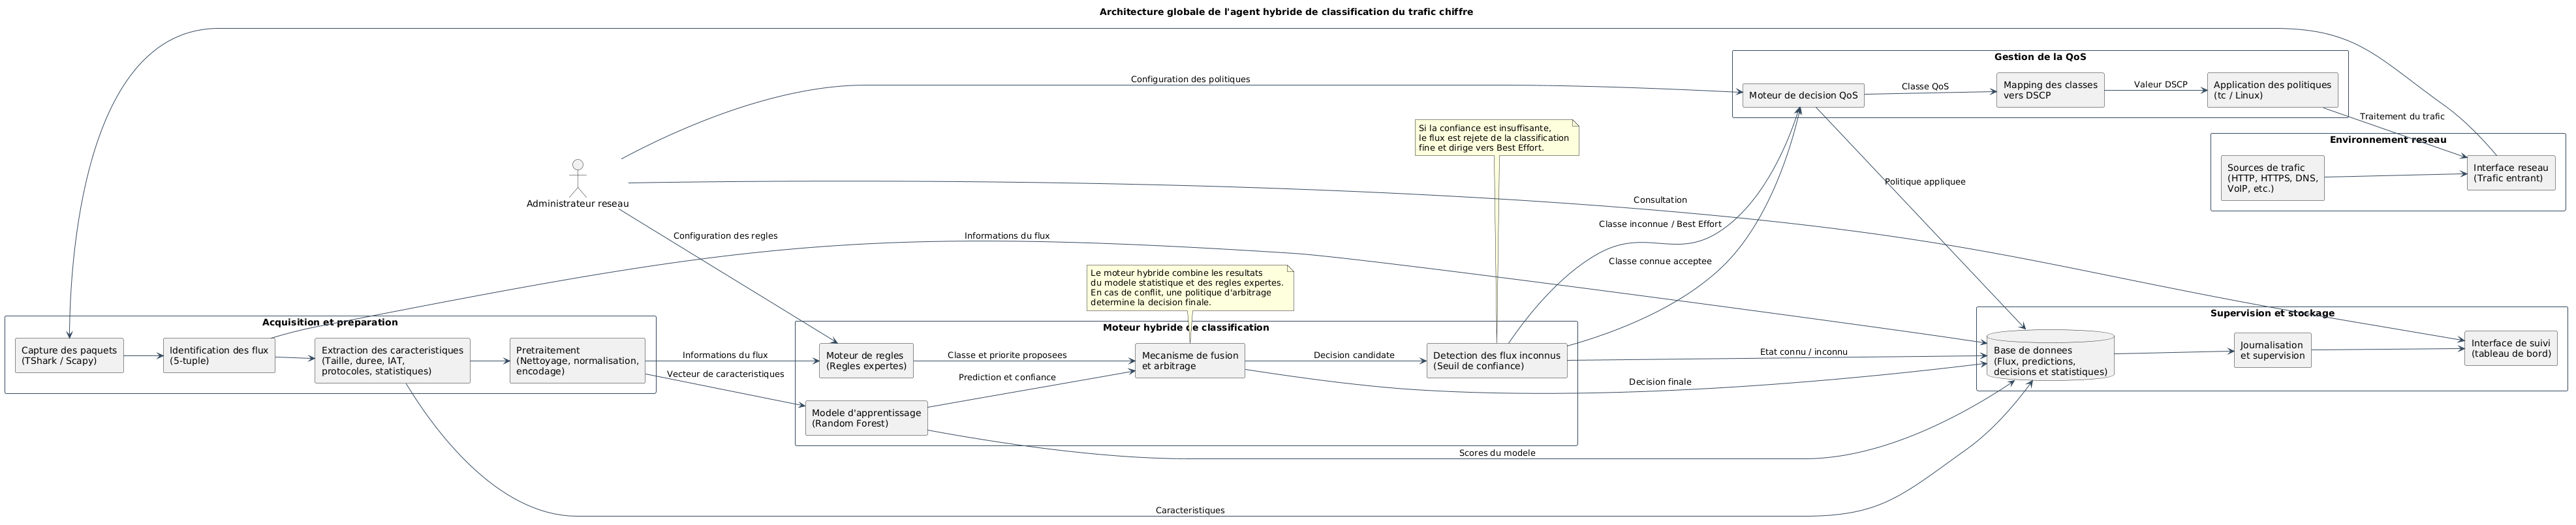
\includegraphics[width=0.95\textwidth]
{img/diag/architecture_globale.png}
}{
\fbox{\parbox{0.85\textwidth}{
\centering
\vspace{1cm}
EMPLACEMENT : architecture globale\\
Fichier : img/diag/architecture\_globale.png
\vspace{1cm}
}}
}
\caption{Architecture globale proposée pour l'agent hybride}
\label{fig:architecture_globale}
\end{figure}

\subsection{Organisation en couches}

\begin{table}[H]
\centering
\caption{Organisation fonctionnelle de l'architecture}
\label{tab:couches}
\begin{tabularx}{\textwidth}{|l|X|X|}
\hline
\textbf{Couche} & \textbf{Composants} &
\textbf{Responsabilités} \\
\hline
Acquisition &
Capture, gestion des flux &
Observer et identifier le trafic. \\
\hline
Traitement &
Extraction, normalisation &
Produire les caractéristiques exploitables. \\
\hline
Intelligence &
ML, règles symboliques &
Produire des prédictions et des scores. \\
\hline
Décision &
Arbitrage, rejet &
Fusionner les résultats et décider. \\
\hline
Action &
QoS, journalisation &
Appliquer les politiques et enregistrer les décisions. \\
\hline
Explicabilité &
SHAP, justification symbolique &
Expliquer les résultats obtenus. \\
\hline
\end{tabularx}
\end{table}

\subsection{Architecture modulaire}

La séparation des responsabilités permet de limiter
les dépendances entre les composants.

Chaque module possède une interface définie et communique
avec les autres composants au moyen de structures
de données normalisées.

Cette organisation présente plusieurs avantages :

\begin{itemize}
    \item possibilité de remplacer un modèle ML sans
    modifier le moteur de règles ;
    \item possibilité d'ajouter de nouvelles règles
    indépendamment de l'entraînement ;
    \item possibilité de comparer plusieurs stratégies
    d'arbitrage ;
    \item facilité de test et de maintenance ;
    \item possibilité de désactiver temporairement
    certains composants en environnement expérimental.
\end{itemize}

\begin{figure}[H]
\centering
\IfFileExists{img/diag/architecture_modulaire.png}{
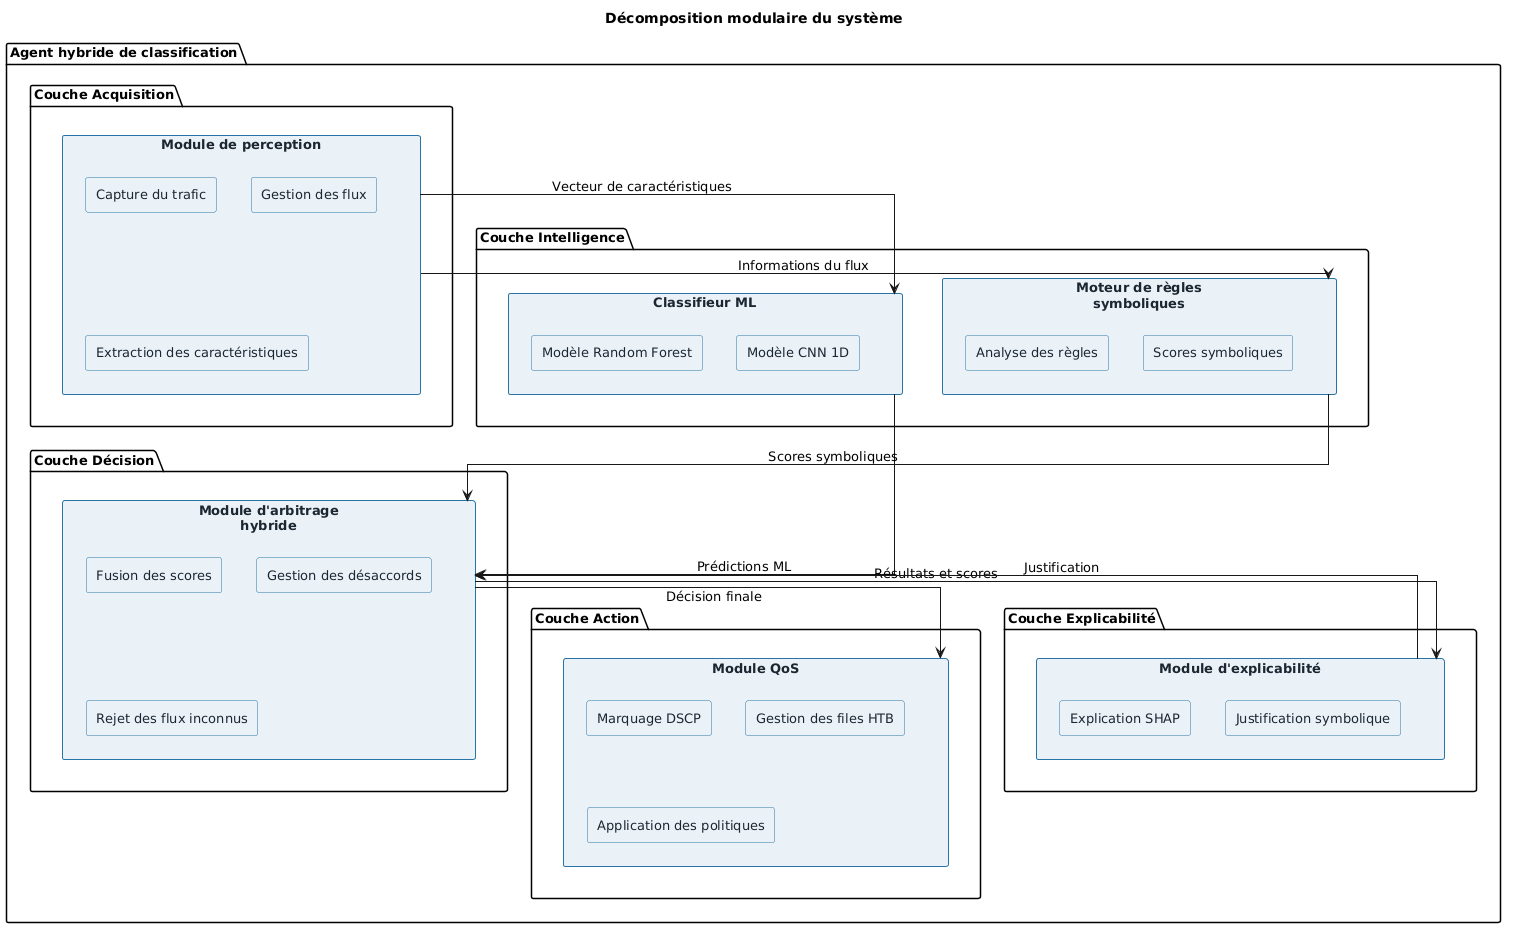
\includegraphics[width=\textwidth]
{img/diag/architecture_modulaire.png}
}{
\fbox{\parbox{0.85\textwidth}{
\centering
\vspace{1cm}
EMPLACEMENT : architecture modulaire\\
Fichier : img/diag/architecture_modulaire.png
\vspace{1cm}
}}
}
\caption{Décomposition modulaire du système}
\label{fig:architecture_modulaire}
\end{figure}

% ------------------------------------------------------------
\section{Conception du module de capture et d'extraction}
% ------------------------------------------------------------

\subsection{Capture du trafic}

Le module de capture constitue le point d'entrée
de l'agent.

Il assure l'observation des paquets circulant sur
une interface réseau déterminée.

TShark peut être utilisé pour effectuer cette opération
et fournir les informations nécessaires au traitement
ultérieur.

Le système ne cherche pas à récupérer le contenu
déchiffré des communications. Il exploite les informations
de transport et les caractéristiques observables.

Les principales opérations sont :

\begin{enumerate}
    \item initialisation de l'interface de capture ;
    \item réception des paquets ;
    \item extraction des champs nécessaires ;
    \item identification de la communication ;
    \item transmission des observations au gestionnaire
    de flux.
\end{enumerate}

\subsection{Identification et gestion des flux}

Un flux est identifié par un ensemble de paramètres
permettant de regrouper les paquets appartenant
à une même communication.

Pour TCP et UDP, une représentation simplifiée
peut être définie par :

\[
F=(IP_s,IP_d,P_s,P_d,Proto)
\]

où :

\begin{itemize}
    \item $IP_s$ : adresse IP source ;
    \item $IP_d$ : adresse IP destination ;
    \item $P_s$ : port source ;
    \item $P_d$ : port destination ;
    \item $Proto$ : protocole de transport.
\end{itemize}

Afin de reconnaître les deux directions d'une communication,
le système utilise une clé canonique ou une association
entre les deux tuples directionnels.

Les flux incomplets, interrompus ou expirés doivent
être traités au moyen de délais d'inactivité configurables.

\subsection{Extraction précoce des caractéristiques}

La classification précoce constitue un élément central
de la conception.

Au lieu d'attendre la fin d'une communication, le système
construit une représentation à partir des $N$ premiers
paquets observés.

On définit :

\[
F_N=\{p_1,p_2,\ldots,p_N\}
\]

où $p_i$ représente le $i$-ème paquet observé.

Le vecteur de caractéristiques peut être défini par :

\[
X_N=(x_1,x_2,\ldots,x_m)
\]

Les caractéristiques envisagées comprennent :

\begin{table}[H]
\centering
\caption{Caractéristiques envisagées pour la représentation des flux}
\label{tab:features}
\begin{tabularx}{\textwidth}{|l|X|X|}
\hline
\textbf{Caractéristique} & \textbf{Description} &
\textbf{Intérêt} \\
\hline
Packet count &
Nombre de paquets observés &
Mesure du volume initial. \\
\hline
Mean packet size &
Taille moyenne des paquets &
Caractérise les échanges. \\
\hline
Standard deviation &
Dispersion des tailles &
Mesure la variabilité. \\
\hline
Inter-arrival time &
Intervalle entre deux paquets &
Caractérise le rythme. \\
\hline
Flow duration &
Durée de la fenêtre observée &
Représente le comportement temporel. \\
\hline
Forward/Backward ratio &
Rapport entre les deux directions &
Caractérise la symétrie des échanges. \\
\hline
Packet size sequence &
Séquence ordonnée des tailles &
Permet une exploitation par CNN 1D. \\
\hline
Transport protocol &
TCP ou UDP &
Apporte un contexte de transport. \\
\hline
\end{tabularx}
\end{table}

La taille moyenne est calculée selon :

\[
\overline{L}=
\frac{1}{N}\sum_{i=1}^{N}L_i
\]

La variance des tailles est :

\[
\sigma_L^2=
\frac{1}{N}\sum_{i=1}^{N}
(L_i-\overline{L})^2
\]

L'intervalle temporel moyen est défini par :

\[
\overline{\Delta t}=
\frac{1}{N-1}
\sum_{i=2}^{N}(t_i-t_{i-1})
\]

Ces indicateurs permettent de représenter le comportement
du flux sans analyser directement son contenu applicatif.

\subsection{Prétraitement des caractéristiques}

Avant leur utilisation par les modèles, les caractéristiques
doivent subir plusieurs opérations :

\begin{itemize}
    \item vérification des valeurs manquantes ;
    \item détection des valeurs non numériques ;
    \item traitement des valeurs infinies ;
    \item normalisation lorsque le modèle l'exige ;
    \item sélection et conservation d'un ordre fixe
    des caractéristiques.
\end{itemize}

Pour une caractéristique normalisée par standardisation :

\[
z_i=\frac{x_i-\mu_i}{\sigma_i}
\]

où $\mu_i$ et $\sigma_i$ représentent respectivement
la moyenne et l'écart-type calculés sur les données
d'entraînement.

Les paramètres du prétraitement doivent être appris
uniquement sur l'ensemble d'entraînement afin d'éviter
les fuites d'information vers les ensembles de validation
et de test.

\subsection{Considérations relatives au chiffrement}

Les protocoles modernes limitent l'exploitation
des informations applicatives.

TLS 1.3 chiffre une grande partie des échanges de négociation.
QUIC s'appuie également sur TLS 1.3 et transporte
les données sur UDP.

Le SNI ou certaines informations DNS peuvent être
exploitables dans certains contextes, mais leur disponibilité
ne doit pas être supposée systématiquement.

L'Encrypted Client Hello (ECH), les mécanismes de
tunneling et les évolutions des protocoles rendent
nécessaire une conception reposant principalement
sur des caractéristiques comportementales.

Ainsi, le système doit fonctionner même lorsque
les métadonnées applicatives sont absentes.

% ------------------------------------------------------------
\section{Conception du module d'apprentissage automatique}
% ------------------------------------------------------------

\subsection{Objectif du classifieur}

Le module ML a pour objectif d'estimer la catégorie
de trafic correspondant au vecteur de caractéristiques
extrait.

Soit l'ensemble des classes connues :

\[
C=\{c_1,c_2,\ldots,c_K\}
\]

Le modèle apprend une fonction :

\[
f_\theta : \mathbb{R}^{m}\rightarrow C
\]

où $\theta$ représente les paramètres appris.

La sortie comprend une classe prédite et, lorsque
le modèle le permet, un vecteur de scores associé
aux différentes classes.

\subsection{Modèle Random Forest}

Random Forest est retenu comme modèle de référence
en raison de sa capacité à exploiter des caractéristiques
numériques et à modéliser des relations non linéaires.

Il s'agit d'une méthode d'ensemble combinant plusieurs
arbres de décision entraînés sur des échantillons
et des sous-ensembles de caractéristiques.

Pour une observation $X$, la prédiction majoritaire
peut être représentée par :

\[
\widehat{y}(X)=
\operatorname{mode}
\{T_1(X),T_2(X),\ldots,T_M(X)\}
\]

où $T_j$ représente le $j$-ième arbre et $M$
le nombre total d'arbres.

La sortie probabiliste brute d'une classe peut être
estimée à partir de la proportion de votes ou des
probabilités agrégées des arbres.

Cependant, ces scores ne doivent pas être considérés
automatiquement comme des probabilités parfaitement
calibrées.

Une étape de calibration pourra être appliquée
sur un ensemble de validation indépendant.

\subsection{Modèle CNN 1D}

En complément du modèle Random Forest, une architecture
CNN 1D peut être envisagée afin d'exploiter les séquences
ordonnées de caractéristiques issues des premiers paquets.

Contrairement à un modèle utilisant uniquement
des statistiques agrégées, un CNN 1D peut apprendre
des motifs locaux dans une séquence.

L'entrée peut être représentée par une matrice :

\[
X\in\mathbb{R}^{N\times d}
\]

où $N$ représente le nombre de paquets observés
et $d$ le nombre de caractéristiques associées
à chaque paquet.

Une architecture simplifiée comprend :

\begin{enumerate}
    \item une couche d'entrée ;
    \item une ou plusieurs couches de convolution 1D ;
    \item une fonction d'activation ReLU ;
    \item une opération de pooling ;
    \item une couche entièrement connectée ;
    \item une couche Softmax pour produire les scores
    des classes.
\end{enumerate}

La convolution peut être représentée par :

\[
Y_{i,j}=
\sum_{k=0}^{r-1}
\sum_{c=1}^{d}
W_{k,c,j}X_{i+k,c}+b_j
\]

où $W$ représente les poids du filtre et $b$
le biais associé.

Le CNN 1D constitue une extension comparative :
son adoption définitive dépendra des ressources
disponibles, de la quantité de données et des résultats
obtenus.

\subsection{Comparaison des deux approches}

\begin{table}[H]
\centering
\caption{Comparaison conceptuelle des modèles}
\label{tab:comparaison_ml}
\begin{tabularx}{\textwidth}{|l|X|X|}
\hline
\textbf{Critère} & \textbf{Random Forest} &
\textbf{CNN 1D} \\
\hline
Entrée &
Caractéristiques statistiques &
Séquences ordonnées. \\
\hline
Complexité &
Modérée &
Plus élevée. \\
\hline
Interprétabilité &
Importance des caractéristiques et SHAP &
Explications plus complexes. \\
\hline
Entraînement &
Généralement plus simple &
Nécessite davantage de réglages. \\
\hline
Utilisation &
Modèle de référence &
Modèle complémentaire. \\
\hline
\end{tabularx}
\end{table}

% ------------------------------------------------------------
\section{Conception du moteur de règles symboliques}
% ------------------------------------------------------------

\subsection{Principe}

Le moteur de règles symboliques représente une source
de connaissance explicite indépendante du modèle ML.

Il applique des conditions prédéfinies sur les métadonnées
et les caractéristiques disponibles.

Chaque règle est définie par :

\[
R_i=(C_i,L_i,w_i)
\]

où :

\begin{itemize}
    \item $C_i$ représente la condition d'activation ;
    \item $L_i$ représente la classe suggérée ;
    \item $w_i$ représente le poids associé à la règle.
\end{itemize}

Une règle peut être représentée par :

\[
C_i(X)=
\begin{cases}
1 & \text{si la condition est satisfaite}\\
0 & \text{sinon}
\end{cases}
\]

Le score symbolique d'une classe peut être calculé
à partir des règles actives :

\[
S_R(c)=
\frac{
\sum_{i:L_i=c}w_iC_i(X)
}{
\sum_i w_iC_i(X)+\varepsilon
}
\]

avec $\varepsilon$ une petite constante évitant
une division par zéro.

Si aucune règle n'est activée, le moteur doit retourner
un état d'absence d'information plutôt qu'une prédiction
arbitraire.

\subsection{Exemples de règles}

\begin{table}[H]
\centering
\caption{Exemples de règles symboliques}
\label{tab:regles}
\begin{tabularx}{\textwidth}{|l|X|X|}
\hline
\textbf{ID} & \textbf{Condition} &
\textbf{Résultat proposé} \\
\hline
R1 &
Métadonnées disponibles correspondant à un service
temps réel connu &
Indice en faveur de VoIP. \\
\hline
R2 &
Caractéristiques temporelles compatibles avec
un flux interactif &
Indice en faveur d'un trafic interactif. \\
\hline
R3 &
Métadonnées applicatives absentes &
Aucune conclusion applicative. \\
\hline
R4 &
Conditions contradictoires entre plusieurs règles &
Signalement d'une ambiguïté. \\
\hline
R5 &
Métadonnées spécifiques et cohérentes avec une
catégorie connue &
Augmentation du score de cette catégorie. \\
\hline
\end{tabularx}
\end{table}

Ces règles constituent des exemples de conception.
Leurs conditions exactes devront être déterminées
à partir des protocoles et des données retenus.

Une règle fondée uniquement sur un port ne doit pas
être considérée comme une preuve suffisante de l'identité
d'une application.

% ------------------------------------------------------------
\section{Conception du moteur d'arbitrage hybride}
% ------------------------------------------------------------

\subsection{Rôle de l'arbitre}

L'arbitre constitue le composant décisionnel central.

Il reçoit les résultats du classifieur ML et du moteur
symbolique, puis détermine une décision unique.

Il doit notamment :

\begin{itemize}
    \item vérifier la disponibilité des deux résultats ;
    \item comparer les classes suggérées ;
    \item combiner les scores disponibles ;
    \item détecter les situations contradictoires ;
    \item évaluer la confiance de la décision ;
    \item déclencher le rejet lorsque les conditions
    de fiabilité ne sont pas satisfaites.
\end{itemize}

\subsection{Formalisation mathématique}

Soit :

\[
P_{ML}(c|X)
\]

la probabilité calibrée estimée par le classifieur ML
pour une classe $c$.

Soit :

\[
S_R(c|X)
\]

le score symbolique normalisé associé à cette classe.

Les poids de fusion sont définis par :

\[
\alpha+\beta=1
\]

avec :

\[
0\leq\alpha\leq1,\qquad
0\leq\beta\leq1
\]

Le score hybride est alors :

\[
S_H(c|X)=
\alpha P_{ML}(c|X)
+
\beta S_R(c|X)
\]

Le score maximal correspond à la classe candidate :

\[
c^*=\arg\max_{c\in C}S_H(c|X)
\]

Cette formulation suppose que les scores ML et symboliques
sont comparables et normalisés. Une calibration ou une
transformation des scores symboliques peut être nécessaire.

\subsection{Prise en compte des désaccords}

La seule maximisation du score hybride ne suffit pas
à caractériser toutes les situations.

L'arbitre doit également mesurer la cohérence
entre les deux sources de décision.

On définit :

\[
A(X)=
\begin{cases}
1 & \text{si les deux modules sont disponibles}\\
0 & \text{sinon}
\end{cases}
\]

Un indicateur de désaccord peut être défini par :

\[
D(X)=
\begin{cases}
0 & \text{si les deux classes sont identiques}\\
1 & \text{sinon}
\end{cases}
\]

Le système peut ensuite appliquer une politique
différenciée :

\begin{itemize}
    \item accord entre les modules : fusion normale ;
    \item désaccord faible : fusion avec pénalité ;
    \item désaccord important : rejet ou décision prudente ;
    \item absence d'un module : fonctionnement dégradé
    explicitement identifié.
\end{itemize}

Il est important de ne pas interpréter une absence
de règle comme une contradiction. Une absence
d'information et une preuve contraire sont deux
situations différentes.

\subsection{Politique de décision}

Soit $\tau$ le seuil minimal de confiance et
$\delta$ un seuil de désaccord.

La décision est définie par :

\[
Decision(X)=
\begin{cases}
c^* & \text{si } S_H(c^*|X)\geq\tau
\text{ et } D(X)<\delta\\
Inconnu & \text{sinon}
\end{cases}
\]

Les seuils $\tau$ et $\delta$ seront déterminés
sur les données de validation.

Cette politique permet de distinguer une prédiction
forte et cohérente d'une décision reposant sur
des informations insuffisantes.

\subsection{Pseudo-code de l'arbitrage}

\begin{algorithm}[H]
\caption{Arbitrage hybride et décision de rejet}
\label{alg:arbitrage}
\begin{algorithmic}[1]

\Require Scores ML, scores symboliques,
poids $\alpha,\beta$, seuil $\tau$

\Ensure Classe finale ou statut Inconnu

\State Vérifier la disponibilité des résultats
\State Normaliser les scores symboliques

\If{le classifieur ML est indisponible}
    \State Retourner le statut de repli défini
\EndIf

\ForAll{$c\in C$}
    \State Calculer :
    \[
    S_H(c)=\alpha P_{ML}(c)+\beta S_R(c)
    \]
\EndFor

\State Déterminer la classe candidate $c^*$

\State Évaluer la cohérence des deux modules

\If{$S_H(c^*)<\tau$}
    \State Retourner \texttt{INCONNU}
\ElsIf{Contradiction importante}
    \State Retourner \texttt{INCONNU}
\Else
    \State Retourner $c^*$
\EndIf

\end{algorithmic}
\end{algorithm}

% ------------------------------------------------------------
\section{Conception du mécanisme de rejet des flux inconnus}
% ------------------------------------------------------------

\subsection{Problématique de la classification en ensemble ouvert}

Un modèle supervisé classique est généralement entraîné
sur un ensemble limité de catégories.

Lorsqu'un nouveau type de trafic apparaît, le modèle
peut néanmoins lui attribuer l'une des catégories
connues, même si cette attribution est incorrecte.

Ce problème correspond à la limite de la classification
en ensemble fermé.

Dans notre système, l'espace des observations peut
comprendre :

\[
\mathcal{X}=
\mathcal{X}_{known}
\cup
\mathcal{X}_{unknown}
\]

Le système doit donc être capable de reconnaître
les observations qui ne sont pas suffisamment
compatibles avec les catégories connues.

\subsection{Mécanisme de rejet}

Le rejet repose sur plusieurs indicateurs :

\begin{itemize}
    \item score maximal du classifieur ;
    \item score hybride ;
    \item écart entre les deux meilleures classes ;
    \item désaccord entre le ML et les règles ;
    \item disponibilité et qualité des caractéristiques.
\end{itemize}

L'écart entre les deux meilleures classes est défini par :

\[
M(X)=S_H(c_1|X)-S_H(c_2|X)
\]

avec $c_1$ et $c_2$ les deux classes présentant
les scores les plus élevés.

Une marge faible peut signaler une ambiguïté entre
plusieurs classes.

Le système peut ainsi utiliser un seuil supplémentaire
sur cette marge afin d'améliorer la prudence des décisions.

\subsection{Calibration des scores}

La calibration est une étape importante car un score
élevé ne correspond pas nécessairement à une confiance
réelle élevée.

La calibration peut être effectuée à l'aide de méthodes
telles que :

\begin{itemize}
    \item calibration sigmoïde ;
    \item calibration isotonic regression.
\end{itemize}

Elle doit être entraînée sur un ensemble de validation
séparé de l'ensemble d'apprentissage.

La qualité de calibration pourra être évaluée
à l'aide des courbes de fiabilité, du Brier Score
et de la log-loss.

\subsection{Politique QoS pour les flux rejetés}

Lorsqu'un flux est classé comme inconnu, le système
ne doit pas lui attribuer automatiquement une priorité
élevée.

La politique recommandée est une classe par défaut
de type Best Effort, soumise aux règles générales
de limitation et de sécurité du réseau.

Le rejet ne signifie pas nécessairement que le flux
est malveillant. Il signifie uniquement que le système
ne dispose pas de suffisamment d'informations fiables
pour lui attribuer une catégorie connue.

% ------------------------------------------------------------
\section{Conception du module d'explicabilité}
% ------------------------------------------------------------

\subsection{Objectif}

L'explicabilité permet de comprendre les facteurs
ayant contribué à une décision de classification.

Le système envisage l'utilisation de SHAP
(\textit{SHapley Additive exPlanations}) afin
d'expliquer les prédictions du modèle ML.

Pour une observation $x$, une explication additive
peut être représentée par :

\[
f(x)=\phi_0+\sum_{i=1}^{m}\phi_i
\]

où :

\begin{itemize}
    \item $\phi_0$ représente la valeur de référence ;
    \item $\phi_i$ représente la contribution de
    la caractéristique $i$ ;
    \item $m$ représente le nombre de caractéristiques.
\end{itemize}

Une valeur positive peut contribuer à augmenter
la prédiction d'une classe, tandis qu'une valeur
négative peut la diminuer, selon la classe expliquée
et la convention utilisée.

\subsection{Explication de la décision hybride}

L'explication globale ne doit pas se limiter
à la sortie SHAP du modèle ML.

Elle doit également intégrer :

\begin{itemize}
    \item les règles activées ;
    \item les règles non satisfaites importantes ;
    \item le score produit par chaque module ;
    \item le niveau de cohérence ;
    \item le seuil appliqué ;
    \item la raison d'un éventuel rejet.
\end{itemize}

Ainsi, une décision pourra être accompagnée
d'une justification structurée.

Exemple :

\begin{quote}
Le flux a été associé à la catégorie VoIP.
Le classifieur ML a fourni un score élevé.
Les règles disponibles apportent des indices cohérents.
Le score hybride dépasse le seuil de décision.
La politique QoS correspondante peut donc être appliquée.
\end{quote}

Pour un flux inconnu, la justification pourra indiquer
que le score est insuffisant ou que les sources
de décision présentent un désaccord important.

% ------------------------------------------------------------
\section{Conception des données}
% ------------------------------------------------------------

\subsection{Modèle conceptuel des données}

Le système doit manipuler les informations relatives
aux flux, aux caractéristiques, aux prédictions,
aux règles, aux décisions et aux politiques QoS.

Les principales entités sont :

\begin{itemize}
    \item Flux ;
    \item Caractéristique ;
    \item Classification ;
    \item Règle ;
    \item Décision ;
    \item Politique QoS.
\end{itemize}

\begin{figure}[H]
\centering
\IfFileExists{img/diag/mcd.png}{
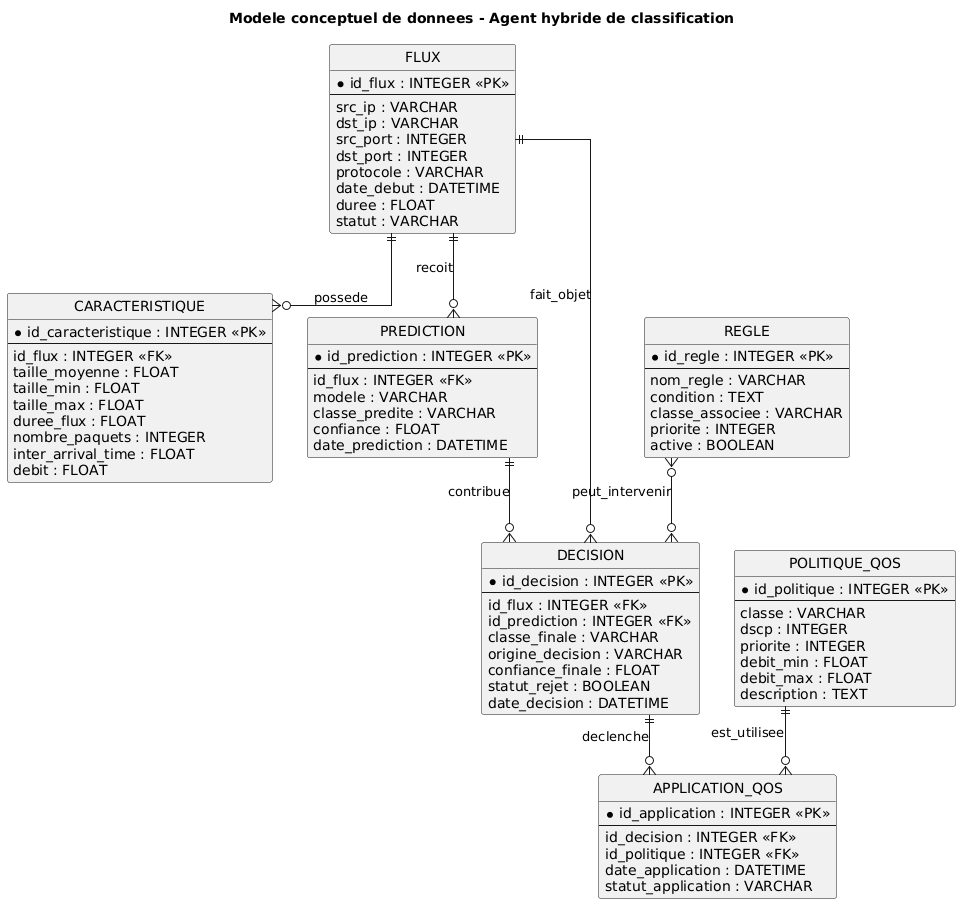
\includegraphics[width=\textwidth]{img/diag/mcd.png}
}{
\fbox{\parbox{0.85\textwidth}{
\centering
\vspace{1cm}
EMPLACEMENT : modèle conceptuel des données\\
Fichier : img/diag/mcd.png
\vspace{1cm}
}}
}
\caption{Modèle conceptuel des données}
\label{fig:mcd}
\end{figure}

\subsection{Description des entités}

\begin{table}[H]
\centering
\caption{Structure conceptuelle des entités}
\label{tab:entites_mcd}
\begin{tabularx}{\textwidth}{|l|X|}
\hline
\textbf{Entité} & \textbf{Attributs proposés} \\
\hline
Flux &
id\_flux, protocole, ip\_source, ip\_destination,
port\_source, port\_destination, date\_debut,
date\_fin. \\
\hline
Caractéristique &
id\_caracteristique, id\_flux, nombre\_paquets,
taille\_moyenne, variance, intervalle\_moyen,
durée\_observation. \\
\hline
Classification &
id\_classification, id\_flux, modèle,
classe\_predite, score, date. \\
\hline
Règle &
id\_regle, condition, classe\_suggeree,
poids, état. \\
\hline
Décision &
id\_decision, id\_flux, classe\_finale,
statut, score\_hybride, justification. \\
\hline
Politique QoS &
id\_politique, classe, DSCP, priorité,
paramètres\_HTB. \\
\hline
\end{tabularx}
\end{table}

\subsection{Relations entre les entités}

Les relations conceptuelles sont définies comme suit :

\begin{itemize}
    \item Un flux possède plusieurs caractéristiques.
    \item Un flux peut faire l'objet de plusieurs classifications.
    \item Plusieurs règles peuvent être évaluées pour un flux.
    \item Un flux peut posséder plusieurs décisions
    enregistrées au cours de son cycle de vie.
    \item Une décision peut être associée à une politique QoS.
    \item Une politique QoS peut être utilisée par
    plusieurs décisions.
\end{itemize}

Cette organisation permet de conserver une traçabilité
entre les observations, les prédictions et les actions
effectuées.

% ------------------------------------------------------------
\section{Conception des interfaces et contrats d'échange}
% ------------------------------------------------------------

\subsection{Principe}

Les modules doivent communiquer au moyen de formats
d'échange cohérents et indépendants de leur implémentation.

Le format JSON est proposé pour les échanges entre
composants lorsque ceux-ci sont exécutés séparément
ou communiquent par une interface structurée.

Les interfaces peuvent également être réalisées
sous forme de fonctions Python si l'architecture
retenue est monolithique.

\subsection{Contrat d'entrée du classifieur}

\begin{verbatim}
{
  "flow_id": "flow_001",
  "protocol": "TCP",
  "packet_count": 10,
  "mean_packet_size": 180.5,
  "std_packet_size": 35.2,
  "mean_interarrival_time": 0.02,
  "duration": 1.8,
  "direction_ratio": 0.65
}
\end{verbatim}

\subsection{Contrat de sortie du classifieur}

\begin{verbatim}
{
  "flow_id": "flow_001",
  "model": "RandomForest",
  "predicted_class": "VoIP",
  "class_scores": {
    "VoIP": 0.92,
    "Video": 0.05,
    "Web": 0.03
  }
}
\end{verbatim}

\subsection{Contrat de sortie du moteur symbolique}

\begin{verbatim}
{
  "flow_id": "flow_001",
  "activated_rules": ["R1", "R2"],
  "suggested_class": "VoIP",
  "rule_score": 0.85,
  "evidence_available": true
}
\end{verbatim}

\subsection{Contrat de sortie de l'arbitre}

\begin{verbatim}
{
  "flow_id": "flow_001",
  "final_class": "VoIP",
  "status": "known",
  "hybrid_score": 0.89,
  "decision_reason": "ML and rules agree",
  "qos_policy": "high_priority"
}
\end{verbatim}

Ces structures constituent des contrats proposés.
Elles devront être harmonisées entre les modules
au début de la phase d'implémentation.

Les scores doivent conserver une signification précise :
probabilité calibrée, score de règle ou score hybride.
Ils ne doivent pas être mélangés sans normalisation.

% ------------------------------------------------------------
\section{Conception de la couche QoS}
% ------------------------------------------------------------

\subsection{Objectif}

La couche QoS exploite la décision finale afin
d'appliquer une politique de traitement adaptée
à la catégorie de trafic.

La qualité de service repose sur plusieurs paramètres,
notamment :

\begin{itemize}
    \item latence ;
    \item gigue ;
    \item débit ;
    \item taux de pertes ;
    \item répartition des ressources réseau.
\end{itemize}

\subsection{Marquage DSCP}

Le champ DSCP est défini dans le champ Differentiated
Services des en-têtes IPv4 et IPv6.

Il utilise six bits pour identifier un codepoint
associé à un comportement de traitement par saut
(\textit{Per-Hop Behavior}).

La valeur DSCP peut être utilisée par les équipements
réseau afin de sélectionner une politique de traitement.

La correspondance entre les classes applicatives
et les valeurs DSCP relève toutefois de la politique
de l'administrateur réseau.

\subsection{Gestion des files HTB}

HTB (\textit{Hierarchical Token Bucket}) permet
d'organiser les classes de trafic et de contrôler
la bande passante attribuée.

Le système peut utiliser une hiérarchie de classes
pour séparer les catégories de trafic.

Une organisation conceptuelle peut être définie :

\begin{itemize}
    \item classe racine ;
    \item classe prioritaire pour les communications
    temps réel validées ;
    \item classe intermédiaire pour la vidéo ;
    \item classe standard pour le trafic Web ;
    \item classe Best Effort pour les flux inconnus.
\end{itemize}

Les paramètres de débit, de plafond et de priorité
seront déterminés expérimentalement.

\subsection{Table de correspondance indicative}

\begin{table}[H]
\centering
\caption{Politique QoS conceptuelle}
\label{tab:politique_qos}
\begin{tabularx}{\textwidth}{|l|l|X|}
\hline
\textbf{Catégorie} & \textbf{Traitement} &
\textbf{Objectif} \\
\hline
VoIP validé &
Priorité élevée &
Limiter la latence et la gigue. \\
\hline
Vidéo &
Bande passante adaptée &
Préserver la fluidité. \\
\hline
Web &
File standard &
Assurer un traitement équilibré. \\
\hline
Inconnu &
Best Effort &
Éviter une priorité non justifiée. \\
\hline
\end{tabularx}
\end{table}

Il convient de préciser que le marquage DSCP ne garantit
pas à lui seul une qualité de service de bout en bout.
Les équipements traversés doivent appliquer une politique
compatible.

% ------------------------------------------------------------
\section{Conception des diagrammes UML}
% ------------------------------------------------------------

\subsection{Diagramme de composants}

Le diagramme de composants présente les unités logicielles
et leurs relations.

Il doit montrer les interfaces entre :

\begin{itemize}
    \item capture réseau ;
    \item extraction des caractéristiques ;
    \item classifieur ML ;
    \item moteur de règles ;
    \item arbitre ;
    \item module SHAP ;
    \item gestionnaire QoS ;
    \item journalisation.
\end{itemize}

\begin{figure}[H]
\centering
\IfFileExists{img/diag/diagramme_composants.png}{
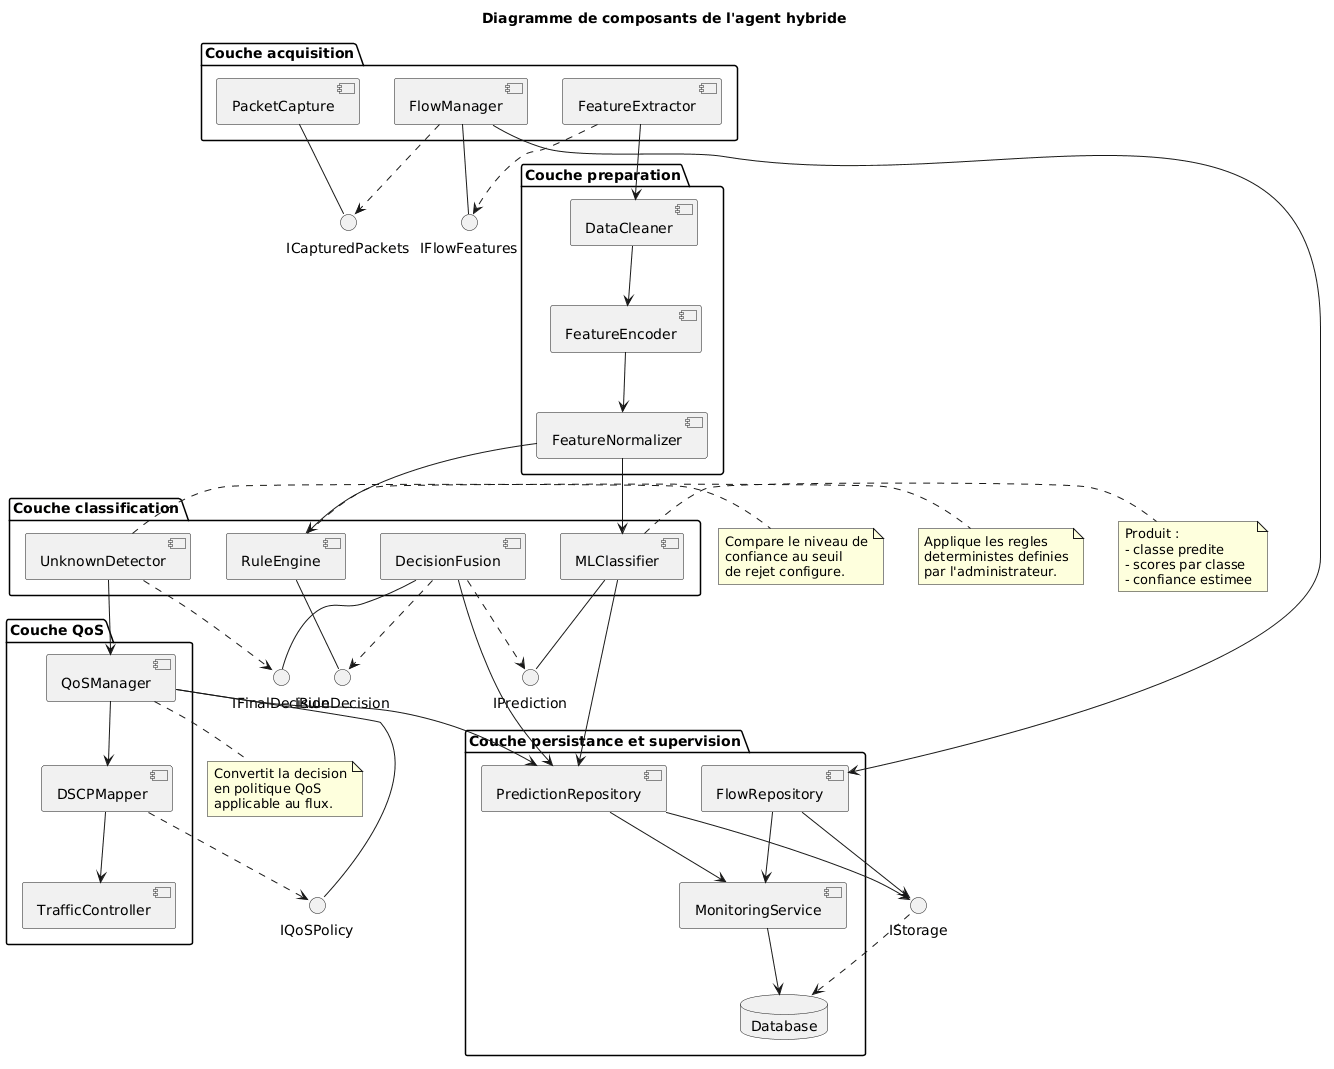
\includegraphics[width=\textwidth]
{img/diag/diagramme_composants.png}
}{
\fbox{\parbox{0.85\textwidth}{
\centering
\vspace{1cm}
EMPLACEMENT : diagramme de composants UML\\
Fichier : img/diag/diagramme\_composants.png
\vspace{1cm}
}}
}
\caption{Diagramme de composants de l'agent hybride}
\label{fig:composants}
\end{figure}

\subsection{Diagramme de déploiement}

Le diagramme de déploiement représente l'environnement
d'exécution du système.

Il doit identifier :

\begin{itemize}
    \item l'interface réseau de capture ;
    \item l'environnement Linux ;
    \item le processus de l'agent Python ;
    \item les fichiers des modèles ML ;
    \item le moteur de règles ;
    \item le mécanisme Linux TC ;
    \item l'environnement Mininet lorsque celui-ci
    est utilisé pour l'expérimentation.
\end{itemize}

\begin{figure}[H]
\centering
\IfFileExists{img/diag/diagramme_deploiement.png}{
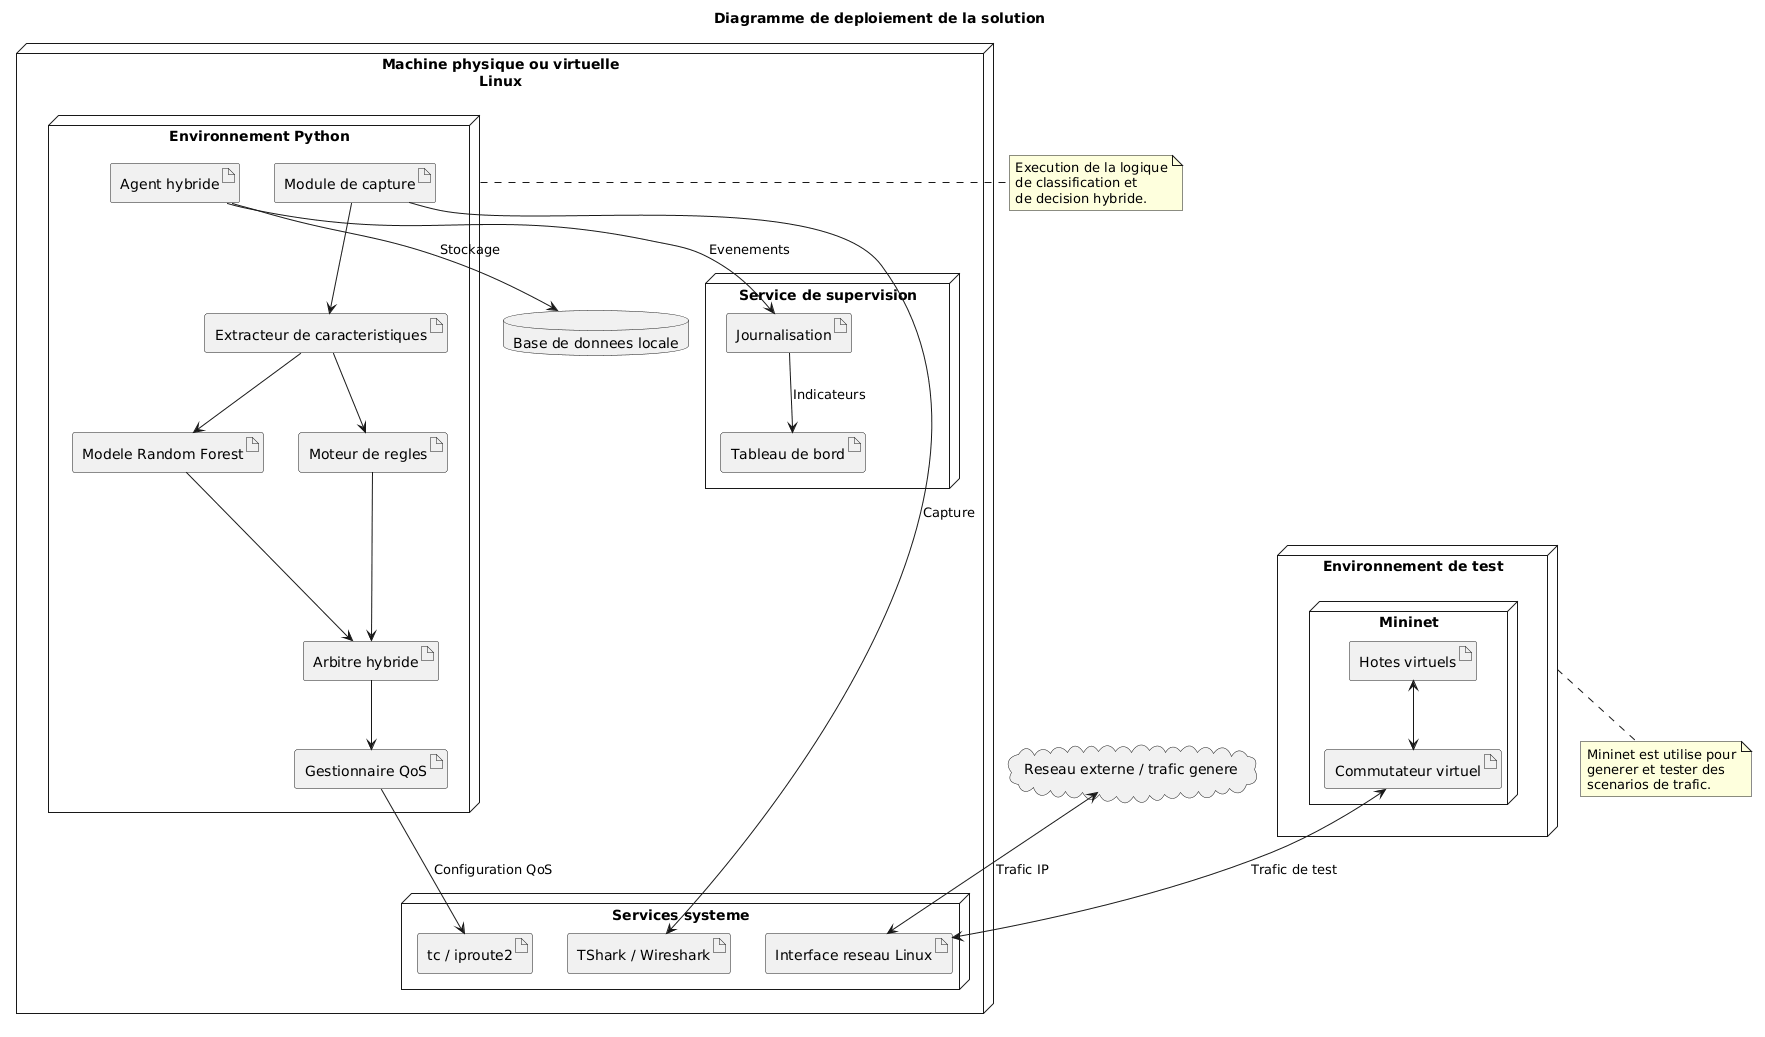
\includegraphics[width=0.95\textwidth]
{img/diag/diagramme_deploiement.png}
}{
\fbox{\parbox{0.85\textwidth}{
\centering
\vspace{1cm}
EMPLACEMENT : diagramme de déploiement UML\\
Fichier : img/diag/diagramme\_deploiement.png
\vspace{1cm}
}}
}
\caption{Diagramme de déploiement de la solution}
\label{fig:deploiement}
\end{figure}

\subsection{Diagramme de séquence de classification}

Ce diagramme décrit l'interaction entre les composants
lorsqu'un flux connu est traité.

\begin{figure}[H]
\centering
\IfFileExists{img/diag/sequence_classification.png}{
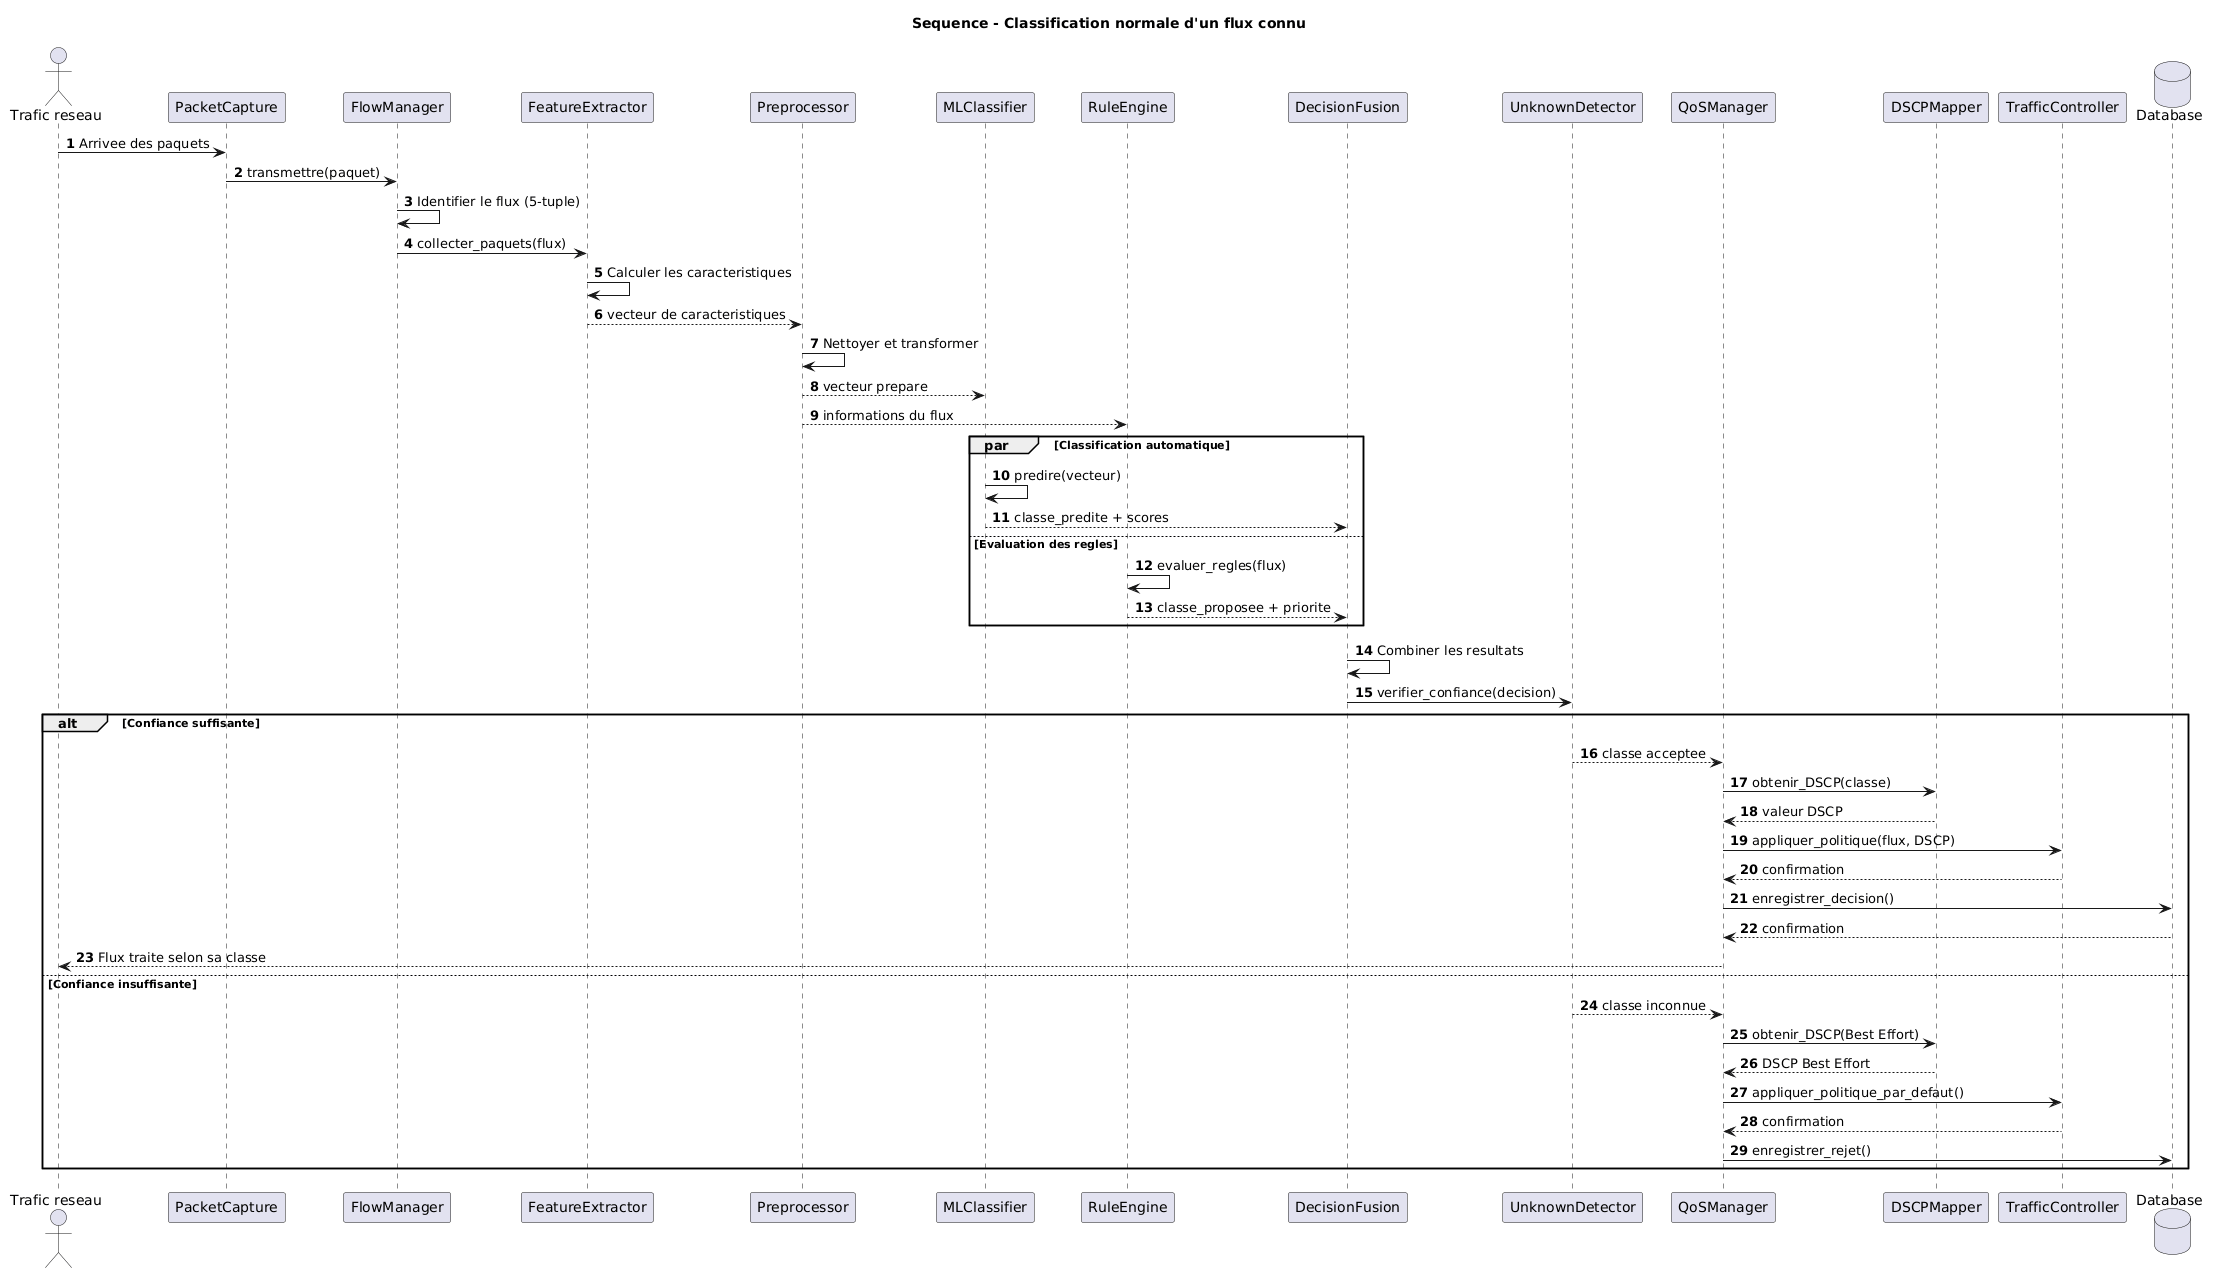
\includegraphics[width=\textwidth]
{img/diag/sequence_classification.png}
}{
\fbox{\parbox{0.85\textwidth}{
\centering
\vspace{1cm}
EMPLACEMENT : séquence de classification\\
Fichier : img/diag/sequence\_classification.png
\vspace{1cm}
}}
}
\caption{Séquence de classification d'un flux connu}
\label{fig:sequence}
\end{figure}

\subsection{Diagramme de séquence du rejet}

Ce diagramme représente le cas dans lequel les scores
ne permettent pas d'identifier une catégorie connue
avec un niveau de confiance suffisant.

\begin{figure}[H]
\centering
\IfFileExists{img/diag/sequence_rejet.png}{
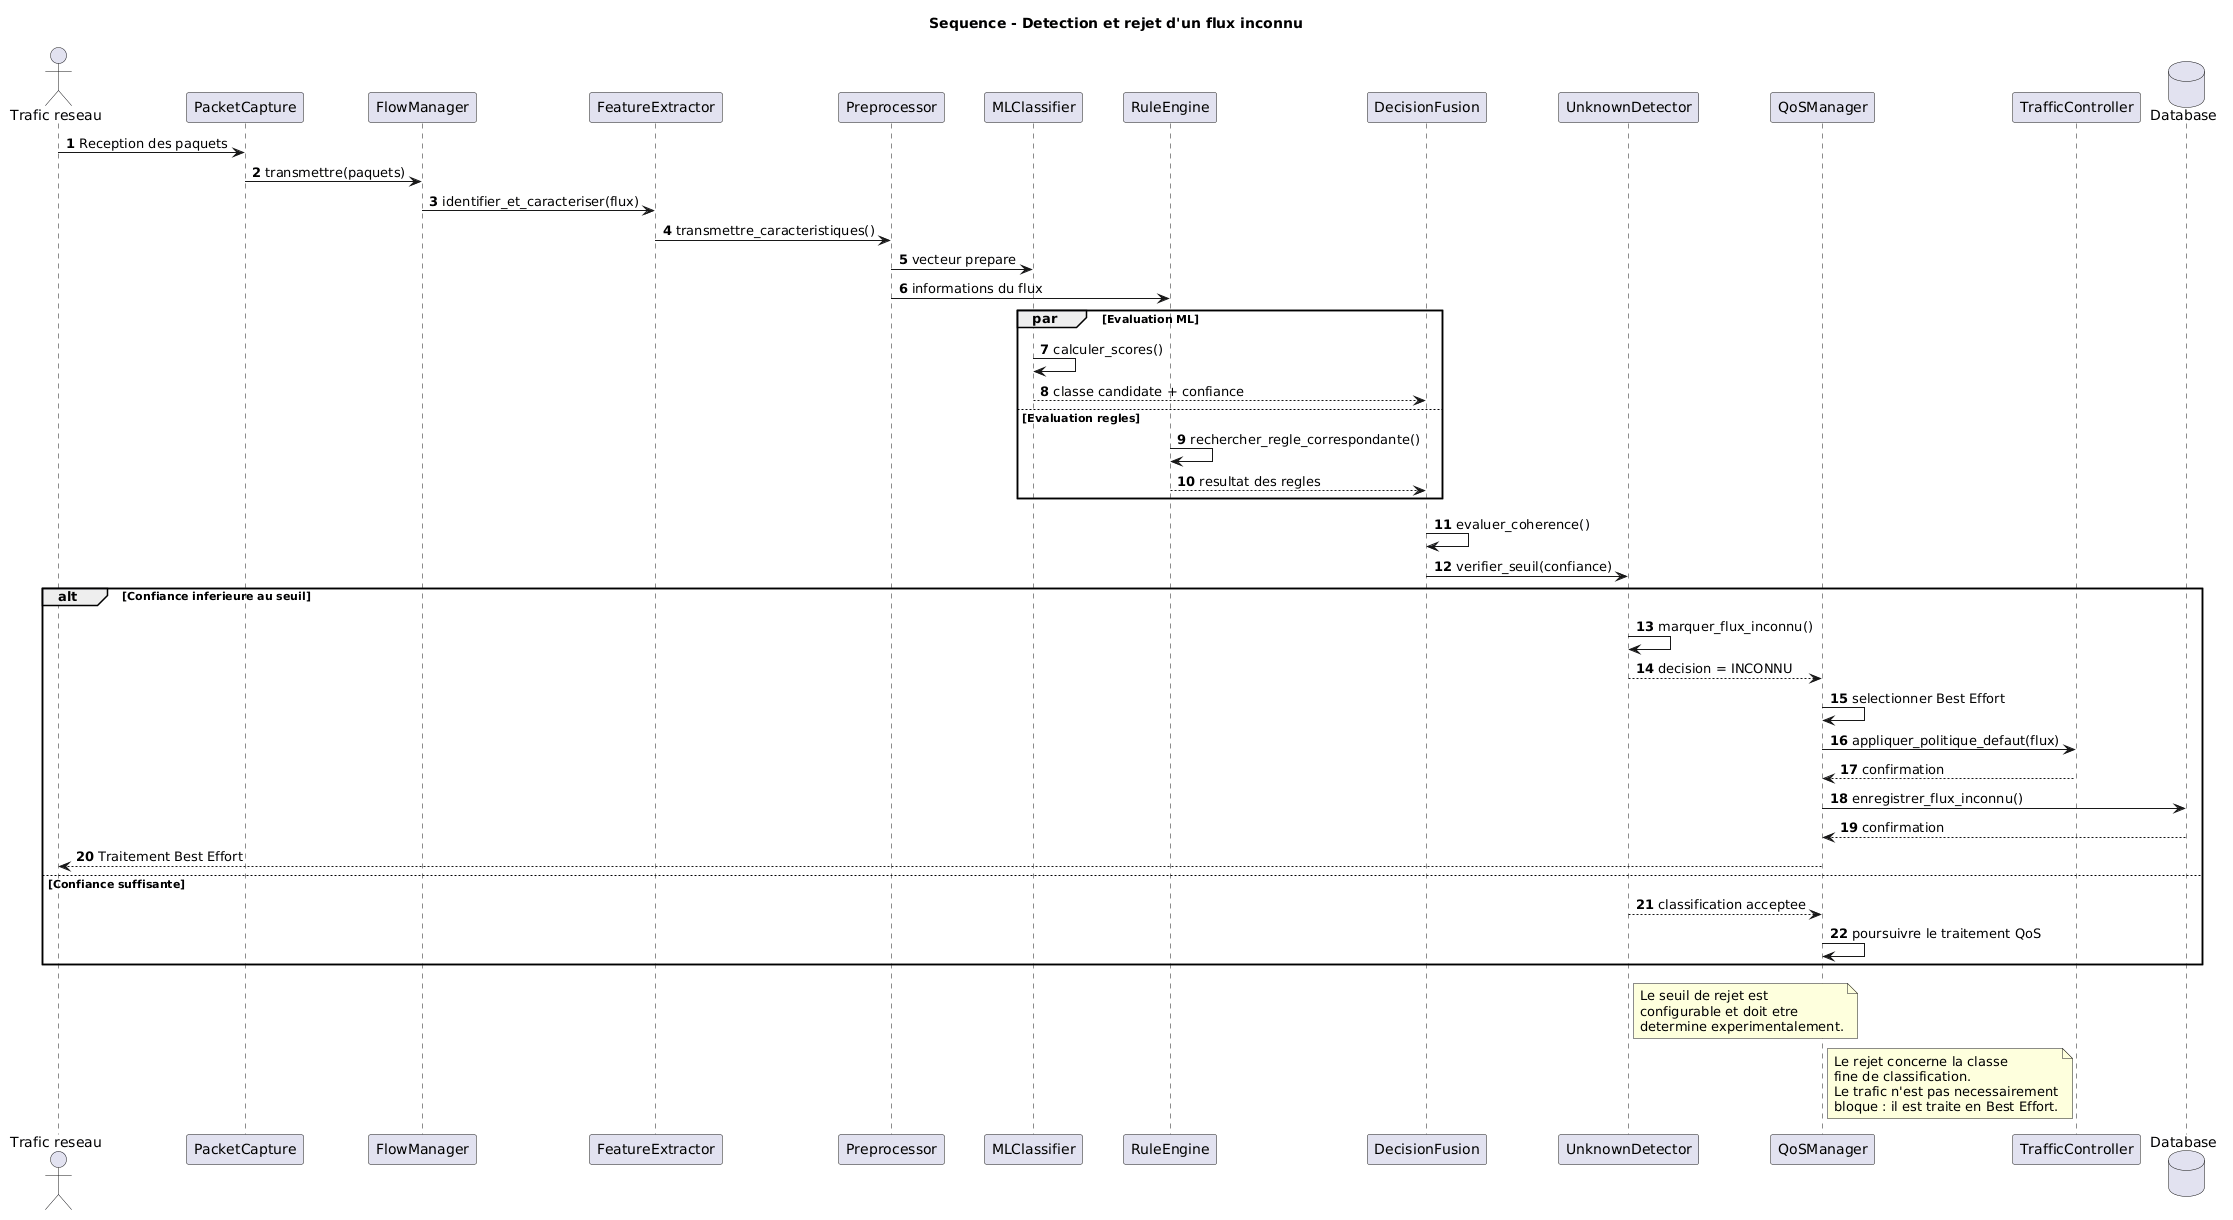
\includegraphics[width=\textwidth]
{img/diag/sequence_rejet.png}
}{
\fbox{\parbox{0.85\textwidth}{
\centering
\vspace{1cm}
EMPLACEMENT : séquence de rejet\\
Fichier : img/diag/sequence\_rejet.png
\vspace{1cm}
}}
}
\caption{Séquence de rejet d'un flux inconnu}
\label{fig:sequence_rejet}
\end{figure}

% ------------------------------------------------------------
\section{Sécurité, fiabilité et gestion des erreurs}
% ------------------------------------------------------------

\subsection{Sécurité de la capture}

La capture réseau nécessite des privilèges particuliers.
Il est recommandé de limiter les privilèges du composant
de capture et de ne pas exécuter inutilement l'ensemble
de l'application avec des droits administrateur.

Les données collectées doivent être limitées aux
informations nécessaires à l'expérimentation.

\subsection{Sécurité de l'application QoS}

La modification des règles réseau doit être effectuée
par un composant disposant des privilèges nécessaires.

Les commandes de configuration ne doivent pas être
construites directement à partir de données non validées
issues des paquets.

Une liste de politiques autorisées doit être définie
afin d'éviter l'exécution de commandes arbitraires.

\subsection{Gestion des erreurs}

\begin{table}[H]
\centering
\caption{Stratégies de gestion des erreurs}
\label{tab:erreurs}
\begin{tabularx}{\textwidth}{|l|X|}
\hline
\textbf{Erreur} & \textbf{Comportement prévu} \\
\hline
Paquets insuffisants &
Poursuivre l'observation ou déclarer une décision
différée. \\
\hline
Caractéristiques manquantes &
Appliquer le prétraitement prévu ou signaler
une observation invalide. \\
\hline
Échec du modèle ML &
Signaler l'indisponibilité et appliquer le mode
de repli défini. \\
\hline
Absence de règle &
Ne pas inventer de classe symbolique. \\
\hline
Désaccord important &
Déclencher la politique de rejet. \\
\hline
Échec QoS &
Journaliser l'échec et conserver la politique
réseau de repli. \\
\hline
Saturation du système &
Limiter la charge et éviter la perte silencieuse
des observations. \\
\hline
\end{tabularx}
\end{table}

% ------------------------------------------------------------
\section{Protocole expérimental et stratégie d'évaluation}
% ------------------------------------------------------------

\subsection{Principe de comparaison}

La conception prévoit trois configurations expérimentales
afin d'isoler la contribution de chaque composant.

\begin{table}[H]
\centering
\caption{Configurations expérimentales}
\label{tab:configurations}
\begin{tabularx}{\textwidth}{|l|X|}
\hline
\textbf{Configuration} & \textbf{Description} \\
\hline
IA seule &
Classification réalisée uniquement par le modèle
d'apprentissage. \\
\hline
Règles seules &
Classification réalisée uniquement par les règles
symboliques. \\
\hline
Approche hybride &
Combinaison du modèle ML, des règles, de l'arbitrage
et du rejet des inconnus. \\
\hline
\end{tabularx}
\end{table}

Cette comparaison permet de déterminer si l'approche
hybride apporte une amélioration par rapport aux
approches prises individuellement.

\subsection{Stratégie de constitution des données}

Les données doivent être séparées en ensembles
d'entraînement, de validation et de test.

Une séparation aléatoire au niveau des lignes peut
produire une fuite d'information lorsque plusieurs
enregistrements proviennent d'une même capture
ou d'une même communication.

Il est donc préférable de réaliser une séparation
par flux, session, capture ou période temporelle
selon la structure du jeu de données.

Les flux inconnus utilisés pour évaluer le rejet
ne doivent pas être présents dans l'entraînement
du classifieur fermé.

\subsection{Métriques de classification}

La précision globale est définie par :

\[
Accuracy=
\frac{TP+TN}{TP+TN+FP+FN}
\]

La précision d'une classe est :

\[
Precision=
\frac{TP}{TP+FP}
\]

Le rappel est :

\[
Recall=
\frac{TP}{TP+FN}
\]

Le score F1 est :

\[
F1=
2\frac{Precision\times Recall}
{Precision+Recall}
\]

Dans un contexte multiclasse, les mesures macro
et pondérées doivent être rapportées afin de tenir
compte des déséquilibres éventuels entre catégories.

\subsection{Métriques du rejet}

L'évaluation du mécanisme de rejet doit distinguer
les flux connus correctement acceptés, les flux
connus rejetés à tort et les flux inconnus correctement
rejetés.

Les indicateurs envisagés comprennent :

\begin{itemize}
    \item taux de rejet des flux inconnus ;
    \item taux de fausse acceptation des inconnus ;
    \item taux de rejet des flux connus ;
    \item précision des décisions acceptées ;
    \item couverture du système.
\end{itemize}

La couverture correspond à la proportion des observations
pour lesquelles le système accepte de fournir
une classe connue.

Elle peut être définie par :

\[
Coverage=
\frac{N_{\text{acceptes}}}
{N_{\text{total}}}
\]

Une bonne stratégie de rejet doit être évaluée
en tenant compte simultanément de la qualité
des classifications acceptées et du taux de couverture.

\subsection{Évaluation des performances temporelles}

La classification précoce implique une attention
particulière au temps de traitement.

Les mesures à effectuer comprennent :

\begin{itemize}
    \item temps moyen de classification ;
    \item temps de traitement par flux ;
    \item nombre de flux traités par seconde ;
    \item mémoire consommée ;
    \item nombre de paquets nécessaires à la décision.
\end{itemize}

\subsection{Évaluation de la QoS}

L'évaluation de la couche QoS doit comparer les
conditions réseau avec et sans application des
politiques.

Les mesures comprennent :

\begin{itemize}
    \item latence moyenne ;
    \item gigue ;
    \item débit par catégorie ;
    \item taux de pertes ;
    \item équité de répartition des ressources.
\end{itemize}

Mininet peut être utilisé pour construire un
environnement réseau contrôlé et reproduire
des conditions de trafic comparables.

Il est important de distinguer la qualité de
classification de l'amélioration effective de
la qualité de service : une bonne précision ML
ne garantit pas à elle seule une amélioration
de la latence ou de la gigue.

\subsection{Limites expérimentales}

Les résultats obtenus dépendront de la représentativité
des données, du nombre de classes, de la diversité
des applications et des conditions de capture.

Les changements de comportement des applications,
les évolutions protocolaires et les mécanismes
de chiffrement peuvent modifier la distribution
des caractéristiques.

Une évaluation temporelle et une analyse des flux
inconnus sont donc nécessaires pour éviter de
surestimer la capacité de généralisation du système.





% ============================================================
% COMPLEMENTS A LA CONCEPTION TECHNIQUE
% A INSERER AVANT LA SECTION CONCLUSION
% ============================================================

% ------------------------------------------------------------
\section{Orchestration et responsabilités détaillées des modules}
% ------------------------------------------------------------

\subsection{Responsabilités des composants}

Afin de garantir une séparation claire des responsabilités,
chaque composant possède une fonction principale et une
interface d'échange définie.

\begin{table}[H]
\centering
\caption{Responsabilités détaillées des composants}
\label{tab:responsabilites_modules}
\begin{tabularx}{\textwidth}{|l|X|X|}
\hline
\textbf{Composant} & \textbf{Responsabilité} & \textbf{Sortie principale} \\
\hline
Capture & Observer les paquets réseau. & Observations horodatées. \\
\hline
Gestionnaire de flux & Regrouper les paquets et gérer les délais. & État du flux. \\
\hline
Extracteur & Calculer les caractéristiques statistiques. & Vecteur de caractéristiques. \\
\hline
Préprocesseur & Vérifier et normaliser les caractéristiques. & Vecteur préparé. \\
\hline
Orchestrateur & Déclencher les moteurs ML et symbolique. & Résultats associés au flux. \\
\hline
Classifieur ML & Produire les scores des classes. & Résultat ML. \\
\hline
Moteur symbolique & Évaluer les règles applicables. & Résultat symbolique. \\
\hline
Arbitre & Fusionner les résultats et décider. & Décision finale. \\
\hline
Gestionnaire QoS & Appliquer une politique autorisée. & Résultat QoS. \\
\hline
Journalisation & Conserver les événements utiles. & Traces horodatées. \\
\hline
\end{tabularx}
\end{table}

\subsection{Rôle de l'orchestrateur}

Le module de capture ne doit pas être responsable de
l'exécution directe des algorithmes de classification.
Il transmet les observations au gestionnaire de flux.
Après extraction et prétraitement, l'orchestrateur
transmet le même vecteur de caractéristiques au
classifieur ML et au moteur symbolique.

Lorsque l'implémentation le permet, ces deux traitements
peuvent être exécutés en parallèle. L'orchestrateur
associe chaque réponse à un identifiant de flux et à
un identifiant de fenêtre d'observation.

Il vérifie les délais de réponse et transmet à l'arbitre
les résultats disponibles ainsi que leur état :
disponible, absent, invalide ou expiré.

\subsection{Cycle de traitement}

\begin{enumerate}
    \item Capture des paquets.
    \item Identification et mise à jour du flux.
    \item Extraction des caractéristiques.
    \item Vérification et prétraitement.
    \item Exécution des moteurs ML et symbolique.
    \item Fusion des résultats par l'arbitre.
    \item Application éventuelle de la politique QoS.
    \item Journalisation de la décision et de ses justifications.
\end{enumerate}

% ------------------------------------------------------------
\section{Politique d'arbitrage et cas de fonctionnement}
% ------------------------------------------------------------

\subsection{Distinction entre absence d'information et contradiction}

Une règle non activée ne constitue pas une preuve contre
une classe. Le moteur symbolique doit distinguer quatre états :

\begin{itemize}
    \item \texttt{SUPPORT} : des règles soutiennent une classe ;
    \item \texttt{CONTRADICTION} : une règle fiable soutient
    explicitement une classe incompatible ;
    \item \texttt{NO\_EVIDENCE} : aucune règle pertinente
    n'est disponible ;
    \item \texttt{ERROR} : le moteur rencontre une défaillance.
\end{itemize}

Cette distinction évite de confondre une absence de métadonnées
DNS ou SNI avec une contradiction.

\subsection{Table de décision de l'arbitre}

\begin{table}[H]
\centering
\caption{Comportement attendu selon les résultats}
\label{tab:decision_arbitre}
\begin{tabularx}{\textwidth}{|l|l|X|}
\hline
\textbf{Résultat ML} & \textbf{Résultat symbolique} &
\textbf{Décision attendue} \\
\hline
Confiant & Soutien de la même classe &
Accepter si les seuils sont atteints. \\
\hline
Confiant & Aucune preuve &
Utiliser le mode ML seul uniquement s'il est autorisé et validé. \\
\hline
Incertain & Soutien symbolique fiable &
Utiliser une règle de secours validée, sinon rejeter. \\
\hline
Disponible & Contradiction explicite &
Retourner \texttt{UNKNOWN}. \\
\hline
Indisponible & Résultat symbolique disponible &
Utiliser le mode symbolique seul uniquement s'il est validé. \\
\hline
Indisponible & Aucune preuve ou erreur &
Retourner \texttt{UNKNOWN}. \\
\hline
\end{tabularx}
\end{table}

\subsection{Normalisation des scores}

La fusion pondérée est valide uniquement si les scores
ML et symboliques sont comparables.

Le score ML doit être calibré sur un ensemble de validation
indépendant. Le score symbolique doit être normalisé
dans l'intervalle $[0,1]$ selon une méthode documentée.

Lorsque les deux sources sont disponibles :

\[
S_H(c|X)=
\alpha P_{ML}(c|X)+\beta S_R(c|X)
\]

avec :

\[
\alpha+\beta=1
\]

En revanche, lorsqu'aucune règle n'est activée, il ne faut
pas automatiquement interpréter le score symbolique nul
comme une contradiction. Le système doit passer dans
un mode dégradé explicitement défini.

\subsection{Critères d'acceptation}

Une classe candidate peut être acceptée lorsque :

\begin{itemize}
    \item les caractéristiques sont valides ;
    \item la fenêtre d'observation est suffisante ;
    \item le score hybride maximal dépasse le seuil $\tau$ ;
    \item la marge entre les deux meilleures classes dépasse
    le seuil $\mu$ ;
    \item aucune contradiction symbolique fiable n'est détectée.
\end{itemize}

La marge est définie par :

\[
M(X)=S_H(c_1|X)-S_H(c_2|X)
\]

où $c_1$ et $c_2$ sont les deux classes présentant
les scores hybrides les plus élevés.

Les seuils $\tau$ et $\mu$, ainsi que les poids
$\alpha$ et $\beta$, sont déterminés sur les données
de validation puis figés avant le test.

% ------------------------------------------------------------
\section{Spécification détaillée des contrats d'interface}
% ------------------------------------------------------------

\subsection{Conventions générales}

Les interfaces utilisent des noms de champs stables
et des types explicites. Les tailles sont exprimées
en octets, les durées en secondes et les ratios dans
l'intervalle $[0,1]$.

Les valeurs absentes sont représentées explicitement
par \texttt{null}. Elles ne doivent jamais être remplacées
silencieusement par zéro.

Chaque message comporte un identifiant de flux et,
lorsque plusieurs fenêtres sont utilisées, un identifiant
de fenêtre.

\subsection{Contrat du vecteur de caractéristiques}

\begin{verbatim}
{
  "schema_version": "1.0",
  "flow_id": "flow_001",
  "window_id": 1,
  "protocol": "TCP",
  "packet_count": 10,
  "mean_packet_size_bytes": 180.5,
  "std_packet_size_bytes": 35.2,
  "mean_interarrival_seconds": 0.02,
  "duration_seconds": 1.8,
  "direction_ratio": 0.60,
  "sni": null,
  "dns_name": null,
  "missing_features": ["sni", "dns_name"]
}
\end{verbatim}

\subsection{Contrat de sortie du moteur symbolique}

\begin{verbatim}
{
  "schema_version": "1.0",
  "flow_id": "flow_001",
  "window_id": 1,
  "engine_status": "ok",
  "evidence_status": "SUPPORT",
  "activated_rules": ["R1", "R2"],
  "contradicting_rules": [],
  "suggested_class": "VoIP",
  "rule_scores": {
    "VoIP": 0.85,
    "Video": 0.10,
    "Web": 0.05
  }
}
\end{verbatim}

Lorsque aucune règle pertinente n'est activée,
\texttt{evidence\_status} prend la valeur
\texttt{NO\_EVIDENCE} et \texttt{suggested\_class}
vaut \texttt{null}.

\subsection{Contrat de sortie de l'arbitre}

\begin{verbatim}
{
  "schema_version": "1.0",
  "flow_id": "flow_001",
  "window_id": 1,
  "status": "known",
  "final_class": "VoIP",
  "hybrid_score": 0.89,
  "confidence_margin": 0.31,
  "decision_reason": "ML_RULES_AGREE",
  "used_degraded_mode": false,
  "qos_policy_id": "qos_voip"
}
\end{verbatim}

Les valeurs possibles de \texttt{status} sont
\texttt{known} et \texttt{unknown}. Pour une décision
inconnue, \texttt{final\_class} vaut \texttt{null}.

Les raisons de rejet peuvent notamment être :
\texttt{LOW\_CONFIDENCE}, \texttt{CONFLICT},
\texttt{INSUFFICIENT\_FEATURES}, \texttt{MODEL\_ERROR}
ou \texttt{RULE\_ENGINE\_ERROR}.

\subsection{Interfaces logicielles proposées}

Dans une implémentation Python monolithique, les interfaces
peuvent être réalisées sous forme de fonctions typées :

\begin{verbatim}
capture_packets(interface: str) -> Iterator[PacketObservation]

update_flow(packet: PacketObservation) -> FlowState

extract_features(flow: FlowState) -> FeatureVector

preprocess_features(features: FeatureVector) -> ModelInput

predict_ml(model_input: ModelInput) -> MLResult

evaluate_rules(features: FeatureVector) -> RuleResult

arbitrate(ml_result: MLResult,
          rule_result: RuleResult) -> Decision

apply_qos(decision: Decision) -> QoSResult

log_event(event: AgentEvent) -> None
\end{verbatim}

Ces signatures constituent des contrats proposés.
Les structures de données associées devront être définies
dans l'implémentation.

% ------------------------------------------------------------
\section{Conception relationnelle et persistance des données}
% ------------------------------------------------------------

\subsection{Choix de persistance}

Le modèle conceptuel présenté précédemment décrit les
informations manipulées par l'agent. Si une conservation
durable des flux, prédictions et décisions est nécessaire,
il peut être traduit en schéma relationnel.

Pour une expérimentation courte, les résultats peuvent
également être conservés dans des fichiers CSV ou JSONL.
Le choix final dépend du volume et des besoins de requêtage.

\subsection{Proposition de modèle logique relationnel}

\begin{itemize}
    \item \textbf{FLUX}(\underline{id\_flux}, protocole,
    ip\_source, ip\_destination, port\_source,
    port\_destination, date\_debut, date\_fin).

    \item \textbf{CARACTERISTIQUE}(\underline{id\_caracteristique},
    \#id\_flux, window\_id, nombre\_paquets,
    taille\_moyenne, variance, intervalle\_moyen,
    duree\_observation).

    \item \textbf{CLASSIFICATION}(\underline{id\_classification},
    \#id\_flux, window\_id, modele, classe\_predite,
    score, date).

    \item \textbf{REGLE}(\underline{id\_regle}, condition,
    classe\_suggeree, poids, etat).

    \item \textbf{DECISION}(\underline{id\_decision},
    \#id\_flux, window\_id, classe\_finale, statut,
    score\_hybride, justification, date).

    \item \textbf{POLITIQUE\_QOS}(\underline{id\_politique},
    classe, dscp, priorite, parametres\_htb).

    \item \textbf{DECISION\_REGLE}(\underline{id\_decision},
    \underline{id\_regle}, resultat\_evaluation).
\end{itemize}

Les attributs soulignés représentent les clés primaires.
Les attributs précédés de \# représentent les clés étrangères.

Une décision peut référencer une politique QoS au moyen
d'un attribut \texttt{id\_politique}, nullable lorsqu'aucune
politique n'a été appliquée.

Ce modèle logique reste une proposition. Les types SQL,
les index et les contraintes physiques seront fixés
lorsque le SGBD sera choisi.

\subsection{Contraintes d'intégrité}

\begin{itemize}
    \item Les identifiants primaires sont uniques et non nuls.
    \item Les ports sont compris entre 0 et 65535.
    \item Les scores normalisés sont compris entre 0 et 1.
    \item Le statut appartient à \texttt{known} ou \texttt{unknown}.
    \item Une décision inconnue ne possède pas de classe finale.
    \item Une politique QoS ne peut être appliquée qu'après
    validation de la décision correspondante.
\end{itemize}

% ------------------------------------------------------------
\section{Gestion des cas limites et modes dégradés}
% ------------------------------------------------------------

\subsection{Métadonnées absentes}

Les champs SNI et DNS ne sont pas garantis. Leur absence
peut résulter de TLS, ECH, QUIC, du DNS chiffré ou de limites
de capture. Le système poursuit donc la classification à
partir des caractéristiques comportementales disponibles.

\subsection{Fenêtre d'observation insuffisante}

Lorsque le nombre de paquets est inférieur au minimum requis,
l'agent peut différer la décision et poursuivre l'observation.
Si le maximum configuré est atteint sans obtenir suffisamment
d'informations, le flux est marqué \texttt{UNKNOWN} avec
la raison \texttt{INSUFFICIENT\_FEATURES}.

\subsection{Flux expiré ou interrompu}

Un flux inactif est clôturé après un délai configurable.
Une décision tardive ne doit pas être appliquée à une
communication qui n'est plus active.

\subsection{Défaillance d'un composant}

Une défaillance ML, symbolique ou QoS doit être représentée
par un statut explicite. Le système applique uniquement
un mode dégradé prévu et validé. À défaut, il conserve
le comportement réseau par défaut et journalise l'erreur.

\subsection{Surcharge et concurrence}

Les états des flux doivent être isolés afin d'éviter
le mélange de caractéristiques. Les files de traitement
doivent être bornées et les délais d'attente configurables.
En cas de surcharge, les pertes d'observation doivent
être signalées.

% ------------------------------------------------------------
\section{Sécurité opérationnelle et traçabilité}
% ------------------------------------------------------------

\subsection{Validation des entrées}

Les champs extraits des paquets sont considérés comme
des données non fiables. Ils sont validés avant leur
utilisation dans les règles, les journaux ou les commandes
de configuration réseau.

Les valeurs numériques doivent être finies et respecter
les plages attendues. Les chaînes doivent être limitées
en taille et correctement échappées lors de leur journalisation.

\subsection{Privilèges minimaux}

La capture et la configuration QoS nécessitent des privilèges
spécifiques. Ces opérations doivent être isolées dans des
composants dédiés disposant uniquement des droits nécessaires.

\subsection{Journal d'audit}

Pour chaque décision, le journal peut conserver :
l'identifiant du flux, l'horodatage, la version du modèle,
la version des règles, les scores, le statut, la raison
d'acceptation ou de rejet et l'action QoS effectivement
exécutée.

% ------------------------------------------------------------
\section{Plan de validation et critères d'acceptation technique}
% ------------------------------------------------------------

\subsection{Tests unitaires et tests d'intégration}

\begin{table}[H]
\centering
\caption{Matrice de validation technique}
\label{tab:validation_technique}
\begin{tabularx}{\textwidth}{|l|X|X|}
\hline
\textbf{Test} & \textbf{Comportement vérifié} &
\textbf{Critère d'acceptation} \\
\hline
Flux connu & Accord ML et règles &
Classe acceptée si les seuils sont atteints. \\
\hline
Flux inconnu & Observation non représentée à l'entraînement &
Statut \texttt{UNKNOWN}. \\
\hline
Désaccord & Classes incompatibles proposées &
Rejet ou mode prudent. \\
\hline
Métadonnées absentes & SNI et DNS indisponibles &
Classification statistique maintenue. \\
\hline
Données invalides & Valeurs non finies ou champs invalides &
Entrée rejetée ou signalée. \\
\hline
Panne d'un moteur & ML ou règles indisponibles &
Mode dégradé explicite. \\
\hline
Échec QoS & Configuration refusée &
Échec journalisé et politique de repli conservée. \\
\hline
Charge élevée & Plusieurs flux simultanés &
Aucune association croisée des flux. \\
\hline
\end{tabularx}
\end{table}

\subsection{Répétabilité des expériences}

Les configurations IA seule, règles seules et hybride
doivent être évaluées sur les mêmes partitions de données.
Les paramètres sont sélectionnés sur la validation et
ne sont plus ajustés sur le test.

Lorsque l'entraînement comporte une part aléatoire,
plusieurs graines sont utilisées et les résultats sont
rapportés sous forme de moyenne et de dispersion.

Les partitions doivent éviter qu'une même communication
ou capture apparaisse simultanément dans l'entraînement
et le test.

\subsection{Analyse complémentaire}

Une étude d'ablation peut mesurer l'effet des règles
symboliques, de l'arbitrage, de la calibration et du rejet.
Les performances doivent être présentées conjointement
avec la couverture, le taux de fausse acceptation des
inconnus et le coût temporel ajouté par l'approche hybride.

Pour la QoS, les mesures doivent être comparées avec
et sans politiques, à charge et topologie identiques.




% ============================================================
% COMPLEMENTS APPROFONDIS DE LA CONCEPTION TECHNIQUE
% A INSERER AVANT LA SECTION CONCLUSION
% ============================================================

% ------------------------------------------------------------
\section{Spécification technique détaillée et fonctionnement interne}
% ------------------------------------------------------------

Cette section approfondit le fonctionnement interne de l'agent hybride. Elle précise les responsabilités des composants, les échanges entre les modules, le cycle de vie d'un flux et les mécanismes permettant de produire une décision cohérente à partir de plusieurs sources d'information.

L'objectif est de passer d'une description architecturale générale à une spécification suffisamment précise pour guider l'implémentation logicielle.

\subsection{Principes de conception logicielle}

La conception repose sur les principes suivants :

\begin{itemize}
    \item \textbf{Séparation des responsabilités :} chaque composant possède une fonction clairement identifiée.
    \item \textbf{Faible couplage :} un module ne doit pas dépendre des détails internes des autres modules.
    \item \textbf{Interfaces explicites :} les échanges reposent sur des structures de données définies.
    \item \textbf{Traçabilité :} chaque décision doit pouvoir être reliée au flux, aux caractéristiques observées et aux résultats des modules.
    \item \textbf{Tolérance aux erreurs :} l'indisponibilité d'un composant ne doit pas provoquer une décision arbitraire.
    \item \textbf{Extensibilité :} de nouveaux modèles, règles ou profils QoS doivent pouvoir être ajoutés sans reconstruire toute l'architecture.
\end{itemize}

La conception distingue trois catégories de composants :

\begin{enumerate}
    \item Les composants d'acquisition et de préparation des données.
    \item Les composants d'analyse et de production des résultats.
    \item Les composants décisionnels et opérationnels.
\end{enumerate}

Cette séparation permet notamment de tester indépendamment l'extraction des caractéristiques, le classifieur, le moteur symbolique et l'arbitre.

\subsection{Responsabilités détaillées des composants}

Le tableau suivant précise les responsabilités attendues de chaque composant.

\begin{table}[H]
\centering
\caption{Spécification détaillée des responsabilités des composants}
\label{tab:responsabilites_detaillees}
\small
\begin{tabularx}{\textwidth}{|l|X|X|}
\hline
\textbf{Composant} & \textbf{Entrées principales} & \textbf{Sorties et responsabilités} \\
\hline
Capture réseau &
Paquets reçus depuis l'interface réseau &
Observations réseau horodatées et transmission au gestionnaire de flux. \\
\hline
Gestionnaire de flux &
Paquets et informations de transport &
Regroupement des paquets, identification des communications et suivi de leur durée de vie. \\
\hline
Extracteur &
Paquets associés à un flux &
Calcul des caractéristiques statistiques, temporelles et directionnelles. \\
\hline
Prétraitement &
Vecteur brut de caractéristiques &
Vérification, transformation et normalisation des données. \\
\hline
Classifieur ML &
Vecteur prétraité &
Classe prédite, scores par classe et informations sur le modèle utilisé. \\
\hline
Moteur symbolique &
Métadonnées disponibles et caractéristiques &
Règles activées, classe suggérée et justification symbolique. \\
\hline
Arbitre &
Résultats ML et symboliques &
Décision finale, score hybride, statut et motif de décision. \\
\hline
Gestionnaire QoS &
Décision finale validée &
Sélection et application d'une politique réseau autorisée. \\
\hline
Journalisation &
Événements et résultats des composants &
Enregistrement des observations, décisions, erreurs et actions. \\
\hline
Explicabilité &
Prédiction ML et informations disponibles &
Contribution des caractéristiques et justification de la décision. \\
\hline
\end{tabularx}
\end{table}

Chaque composant doit exposer une interface stable. Par exemple, le gestionnaire de flux ne doit pas connaître l'architecture interne du modèle Random Forest. Il transmet uniquement un objet contenant les caractéristiques nécessaires au classifieur.

De la même manière, le gestionnaire QoS ne doit pas recalculer la classification. Il reçoit une décision produite par l'arbitre et applique la politique correspondante lorsque les conditions de validation sont satisfaites.

\subsection{Cycle de vie complet d'un flux}

Le traitement d'une communication est organisé sous la forme d'un cycle de vie composé de plusieurs états.

\begin{enumerate}
    \item \textbf{OBSERVED :} un premier paquet correspondant à une nouvelle communication est détecté.
    \item \textbf{COLLECTING :} les paquets suivants sont associés au flux et les informations nécessaires sont accumulées.
    \item \textbf{FEATURES\_READY :} la fenêtre d'observation atteint les conditions nécessaires à l'extraction.
    \item \textbf{ANALYZING :} les modules ML et symbolique réalisent leur analyse.
    \item \textbf{DECIDED :} l'arbitre produit une décision ou un rejet.
    \item \textbf{APPLIED :} la politique QoS correspondante est appliquée, si elle est autorisée.
    \item \textbf{EXPIRED ou CLOSED :} le flux est terminé ou supprimé après expiration.
\end{enumerate}

Le cycle peut être représenté par le modèle conceptuel suivant :

\begin{figure}[H]
\centering
\begin{tabular}{c}
\textbf{OBSERVED} \\
$\downarrow$ \\
\textbf{COLLECTING} \\
$\downarrow$ \\
\textbf{FEATURES\_READY} \\
$\downarrow$ \\
\textbf{ANALYZING} \\
$\downarrow$ \\
\textbf{DECIDED} \\
$\downarrow$ \\
\textbf{APPLIED} \\
$\downarrow$ \\
\textbf{CLOSED / EXPIRED}
\end{tabular}
\caption{Cycle de vie conceptuel d'un flux}
\label{fig:cycle_vie_flux}
\end{figure}

Une transition vers un état d'erreur peut intervenir à différentes étapes. Par exemple, une capture interrompue peut empêcher la constitution d'une fenêtre d'observation suffisante.

Dans ce cas, le système doit enregistrer l'événement et éviter de transmettre au classifieur un vecteur incomplet présenté comme une observation valide.

\subsection{Gestion de l'identité et de l'état des flux}

Chaque flux doit disposer d'un identifiant interne unique, appelé \texttt{flow\_id}.

Cet identifiant permet de relier les différentes opérations réalisées pendant le cycle de vie de la communication.

Une structure logique peut être définie comme suit :

\begin{verbatim}
FlowContext:
    flow_id
    protocol
    source_address
    destination_address
    source_port
    destination_port
    start_timestamp
    last_seen_timestamp
    packet_count
    forward_packets
    backward_packets
    packet_observations
    current_state
    classification_status
\end{verbatim}

Le gestionnaire de flux doit également prendre en compte les communications bidirectionnelles.

Pour éviter de considérer une même communication comme deux flux indépendants, une clé canonique peut être construite à partir des deux extrémités.

Pour un flux TCP ou UDP, une représentation conceptuelle est :

\[
K(F)=\operatorname{canonical}
\left(
(IP_s,P_s),(IP_d,P_d),Proto
\right)
\]

La fonction \texttt{canonical} doit produire une représentation identique quelle que soit la direction du paquet.

Il convient néanmoins de conserver la direction d'origine de chaque paquet afin de calculer les caractéristiques avant et arrière.

Pour les protocoles multiplexés, notamment QUIC, cette identification reste une approximation au niveau transport. Une connexion ne correspond pas nécessairement à une seule activité applicative.

\subsection{Définition des conditions de déclenchement de la classification}

La classification précoce nécessite de définir des conditions précises de déclenchement.

La décision peut être déclenchée lorsque :

\begin{itemize}
    \item le nombre minimal de paquets est atteint ;
    \item la durée minimale d'observation est respectée ;
    \item les caractéristiques obligatoires sont disponibles ;
    \item le vecteur obtenu respecte le schéma attendu par le modèle.
\end{itemize}

On peut définir une condition logique :

\[
Ready(F)=
(N_F\geq N_{\min})
\land
(V_F=1)
\land
(T_F\geq T_{\min})
\]

où :

\begin{itemize}
    \item $N_F$ représente le nombre de paquets observés ;
    \item $N_{\min}$ représente le nombre minimal de paquets ;
    \item $V_F$ indique si le vecteur est valide ;
    \item $T_F$ représente la durée d'observation ;
    \item $T_{\min}$ représente la durée minimale éventuelle.
\end{itemize}

Les paramètres $N_{\min}$ et $T_{\min}$ doivent être déterminés expérimentalement.

Il ne faut pas imposer une durée minimale excessive, car cela réduirait l'intérêt de la classification précoce. À l'inverse, une observation trop courte peut produire des caractéristiques insuffisantes pour distinguer certaines catégories.

% ------------------------------------------------------------
\section{Spécification approfondie du moteur d'arbitrage hybride}
% ------------------------------------------------------------

\subsection{Problématique de la fusion des résultats}

Le classifieur ML et le moteur symbolique peuvent produire des résultats différents pour un même flux.

Cette situation est normale, car les deux mécanismes ne reposent pas sur les mêmes informations.

Le classifieur ML apprend des relations statistiques à partir des données d'entraînement. Le moteur symbolique exploite des connaissances explicites, notamment les métadonnées disponibles et les conditions définies dans les règles.

L'arbitre doit donc éviter une fusion naïve des résultats.

Il doit distinguer :

\begin{itemize}
    \item l'accord entre les deux sources ;
    \item le désaccord entre les deux sources ;
    \item l'absence de résultat symbolique ;
    \item l'indisponibilité d'un composant ;
    \item l'insuffisance de confiance ;
    \item la présence d'indices indiquant une classe inconnue.
\end{itemize}

La décision finale ne doit pas être déterminée uniquement par la valeur numérique la plus élevée.

\subsection{Représentation normalisée des résultats}

Pour permettre une comparaison cohérente, chaque module doit produire un résultat structuré.

Pour le classifieur ML, on définit :

\[
R_{ML}=(\hat{c}_{ML},P_{ML},v_{ML})
\]

où :

\begin{itemize}
    \item $\hat{c}_{ML}$ est la classe prédite ;
    \item $P_{ML}$ est le vecteur des scores associés aux classes ;
    \item $v_{ML}$ indique la validité du résultat.
\end{itemize}

Le vecteur des scores est :

\[
P_{ML}=
\left(
p_1,p_2,\ldots,p_K
\right)
\]

avec :

\[
p_k\in[0,1]
\]

Lorsque les scores sont interprétés comme des probabilités, leur calibration doit être vérifiée.

Pour le moteur symbolique, on définit :

\[
R_R=(\hat{c}_R,S_R,A_R,v_R)
\]

où :

\begin{itemize}
    \item $\hat{c}_R$ est la classe suggérée par les règles ;
    \item $S_R$ est le score symbolique ;
    \item $A_R$ représente l'ensemble des règles activées ;
    \item $v_R$ indique la validité du résultat.
\end{itemize}

L'absence de règle activée doit être représentée explicitement. Elle ne doit pas être interprétée comme une preuve que la classe prédite par le modèle est incorrecte.

\subsection{Normalisation des scores}

Les scores issus des deux mécanismes ne possèdent pas nécessairement la même signification.

Un score ML peut représenter une probabilité estimée, tandis qu'un score symbolique peut représenter une combinaison de poids attribués aux règles.

Il est donc nécessaire de distinguer :

\begin{itemize}
    \item les probabilités produites par le modèle ;
    \item les scores de correspondance des règles ;
    \item les scores de confiance calibrés ;
    \item les scores hybrides calculés par l'arbitre.
\end{itemize}

Si les deux sources doivent être combinées numériquement, une transformation préalable doit être définie.

On peut représenter les scores normalisés par :

\[
\widetilde{P}_{ML}(c)
=
Cal_{ML}(P_{ML}(c))
\]

\[
\widetilde{S}_{R}(c)
=
Norm_R(S_R(c))
\]

La fonction $Cal_{ML}$ correspond à une éventuelle calibration du modèle.

La fonction $Norm_R$ transforme le score symbolique dans une échelle compatible.

Ces transformations doivent être définies et validées sur des données indépendantes de l'ensemble de test.

\subsection{Calcul du score hybride}

Une stratégie de fusion pondérée peut être utilisée lorsque les deux résultats sont valides et comparables.

Le score hybride d'une classe $c$ est défini par :

\[
S_H(c|X)=
\alpha\widetilde{P}_{ML}(c|X)
+
\beta\widetilde{S}_{R}(c|X)
\]

avec :

\[
\alpha+\beta=1
\]

et :

\[
\alpha,\beta\in[0,1]
\]

Les coefficients représentent l'importance attribuée à chaque source.

Ils ne doivent pas être fixés arbitrairement. Leur choix doit être étudié à partir des performances obtenues sur l'ensemble de validation.

Lorsque le moteur symbolique ne dispose d'aucune preuve exploitable, il ne faut pas lui attribuer automatiquement un score nul qui pénaliserait le classifieur.

Dans ce cas, une stratégie de fusion adaptée peut utiliser uniquement le résultat ML valide, tout en indiquant que la décision repose sur une seule source.

\subsection{Gestion de l'accord entre les sources}

Lorsque les deux mécanismes proposent la même classe, l'arbitre peut considérer cette convergence comme un indice favorable.

Cependant, l'accord ne constitue pas une garantie absolue de correction.

Les deux mécanismes peuvent partager des biais ou exploiter des informations insuffisantes.

La décision doit donc également prendre en compte les seuils de confiance et la validité des observations.

On peut définir la condition :

\[
Agreement=
(\hat{c}_{ML}=\hat{c}_R)
\]

Si cette condition est vraie et que les scores dépassent les seuils définis, la classe commune peut être acceptée.

\subsection{Gestion du désaccord}

Lorsque :

\[
\hat{c}_{ML}\neq\hat{c}_R
\]

l'arbitre doit identifier la nature du désaccord.

Plusieurs situations sont possibles :

\begin{itemize}
    \item le modèle ML présente une confiance élevée et les règles sont peu spécifiques ;
    \item les règles présentent une correspondance forte et le modèle ML est incertain ;
    \item les deux mécanismes présentent des scores élevés pour des classes différentes ;
    \item les deux mécanismes présentent des scores faibles.
\end{itemize}

Un désaccord important ne doit pas conduire automatiquement à choisir la classe possédant le score brut le plus élevé.

Une politique conservatrice consiste à rejeter le flux lorsque les sources fournissent des indications incompatibles et suffisamment fortes.

\subsection{Politique de décision proposée}

La politique suivante distingue les situations principales.

\begin{table}[H]
\centering
\caption{Politique détaillée de l'arbitre hybride}
\label{tab:politique_arbitrage_detaillee}
\small
\begin{tabularx}{\textwidth}{|X|X|X|}
\hline
\textbf{Situation} & \textbf{Condition} & \textbf{Décision proposée} \\
\hline
Accord fiable &
Les deux sources proposent la même classe et les seuils sont respectés. &
Accepter la classe commune. \\
\hline
Accord incertain &
Les deux sources proposent la même classe, mais les scores sont insuffisants. &
Rejeter ou différer la décision. \\
\hline
ML seul exploitable &
Le modèle est valide et aucune preuve symbolique exploitable n'est disponible. &
Utiliser le résultat ML si son seuil est satisfait et si la politique l'autorise. \\
\hline
Règles seules exploitables &
Le modèle est indisponible et une règle suffisamment spécifique est activée. &
Appliquer une décision symbolique uniquement si cette stratégie est autorisée. \\
\hline
Désaccord fort &
Les deux sources proposent des classes différentes avec des scores élevés. &
Rejeter la classification ou demander une observation complémentaire. \\
\hline
Scores insuffisants &
Aucune classe ne dépasse le seuil minimal. &
Déclarer le flux inconnu ou incertain. \\
\hline
Erreur de traitement &
Les données ou les résultats d'un composant sont invalides. &
Déclarer une erreur et appliquer le mode de repli. \\
\hline
\end{tabularx}
\end{table}

Cette politique permet de distinguer le rejet d'un flux inconnu du rejet provoqué par une erreur technique.

Ces deux situations doivent posséder des statuts différents dans les journaux.

\subsection{Mécanisme de rejet des flux inconnus}

Le système évolue dans un environnement ouvert. Les catégories réellement observées peuvent donc être différentes de celles présentes dans les données d'entraînement.

Un classifieur traditionnel attribue généralement une classe parmi les catégories connues, même lorsque le flux est très éloigné des données d'apprentissage.

Le mécanisme de rejet vise à limiter ce comportement.

On définit le score maximal :

\[
S_{\max}(X)=\max_{c\in C}S_H(c|X)
\]

On définit également la marge entre les deux meilleurs scores :

\[
M(X)=S_{(1)}(X)-S_{(2)}(X)
\]

où $S_{(1)}$ et $S_{(2)}$ représentent respectivement le premier et le deuxième meilleur score.

Une décision peut être acceptée lorsque :

\[
S_{\max}(X)\geq\tau
\]

et :

\[
M(X)\geq\mu
\]

où :

\begin{itemize}
    \item $\tau$ est le seuil minimal de confiance ;
    \item $\mu$ est la marge minimale entre les deux meilleures classes.
\end{itemize}

Ces deux conditions permettent de distinguer une prédiction suffisamment forte d'une situation dans laquelle plusieurs classes sont difficilement séparables.

Les valeurs de $\tau$ et $\mu$ doivent être déterminées expérimentalement.

Le rejet peut également prendre en compte la cohérence entre les sources, la disponibilité des caractéristiques et les résultats des règles symboliques.

\subsection{Pseudo-code de l'arbitrage}

L'algorithme suivant décrit le fonctionnement logique proposé.

\begin{verbatim}
function arbitrate(ml_result, rule_result, thresholds):

    if not ml_result.valid and not rule_result.valid:
        return ERROR

    if ml_result.valid:
        ml_scores = validate_scores(ml_result.scores)

        if ml_scores.invalid:
            return ERROR

    if rule_result.valid:
        rule_scores = validate_rule_scores(
            rule_result.scores
        )

        if rule_scores.invalid:
            return ERROR

    if ml_result.valid and rule_result.valid:

        ml_class = ml_result.predicted_class
        rule_class = rule_result.suggested_class

        if rule_result.has_evidence:
            scores = normalize_and_fuse(
                ml_result,
                rule_result
            )
        else:
            scores = ml_scores

    elif ml_result.valid:
        scores = ml_scores

    else:
        if rule_result.has_specific_evidence:
            return symbolic_decision(rule_result)
        else:
            return UNKNOWN

    best_class = argmax(scores)
    best_score = max(scores)
    margin = compute_margin(scores)

    if best_score < thresholds.min_score:
        return UNKNOWN

    if margin < thresholds.min_margin:
        return UNCERTAIN

    if sources_strongly_disagree(
        ml_result,
        rule_result
    ):
        return REJECTED

    return ACCEPTED(best_class, best_score)
\end{verbatim}

Ce pseudo-code constitue une spécification fonctionnelle. Les fonctions de normalisation, de fusion et de détection des désaccords doivent être implémentées selon les modèles et les règles effectivement retenus.

% ------------------------------------------------------------
\section{Spécification détaillée des interfaces logicielles}
% ------------------------------------------------------------

\subsection{Objectif des contrats d'interface}

Les interfaces définissent les informations qu'un composant peut recevoir, les résultats qu'il doit retourner et les erreurs qu'il peut signaler.

Elles permettent d'éviter les dépendances implicites entre modules.

Chaque interface doit préciser :

\begin{itemize}
    \item le nom de l'opération ;
    \item les paramètres obligatoires ;
    \item les paramètres facultatifs ;
    \item les types de données ;
    \item les unités utilisées ;
    \item les valeurs autorisées ;
    \item la structure du résultat ;
    \item les erreurs possibles.
\end{itemize}

Les contrats ci-dessous peuvent être utilisés avec des fonctions Python ou avec des échanges JSON.

\subsection{Contrat du gestionnaire de flux}

Le gestionnaire de flux reçoit les observations produites par le module de capture.

Son rôle est de regrouper les paquets, de maintenir l'état des communications et de déclencher l'extraction lorsque les conditions sont satisfaites.

Interface proposée :

\begin{verbatim}
update_flow(packet) -> FlowContext

get_flow(flow_id) -> FlowContext

is_ready(flow_id) -> Boolean

expire_flow(flow_id) -> Boolean

close_flow(flow_id) -> FlowSummary
\end{verbatim}

Les opérations doivent respecter les contraintes suivantes :

\begin{itemize}
    \item Un paquet invalide ne doit pas modifier l'état d'un flux.
    \item Un paquet appartenant à un flux existant doit mettre à jour son horodatage.
    \item Un nouveau flux doit recevoir un identifiant unique.
    \item Un flux expiré ne doit pas être traité comme une communication active.
    \item Les compteurs directionnels doivent rester cohérents avec les paquets observés.
\end{itemize}

\subsection{Contrat de l'extracteur de caractéristiques}

L'extracteur transforme les observations d'un flux en vecteur numérique.

Interface proposée :

\begin{verbatim}
extract_features(flow_context) -> FeatureVector
\end{verbatim}

Le résultat doit contenir les informations suivantes :

\begin{verbatim}
{
    "flow_id": "flow_001",
    "feature_version": "1.0",
    "packet_count": 10,
    "mean_packet_size": 180.5,
    "std_packet_size": 35.2,
    "mean_interarrival_time": 0.02,
    "duration": 1.8,
    "forward_count": 6,
    "backward_count": 4,
    "direction_ratio": 0.60,
    "valid": true
}
\end{verbatim}

Les unités doivent être uniformisées :

\begin{itemize}
    \item tailles des paquets : octets ;
    \item durée : secondes ;
    \item intervalles temporels : secondes ;
    \item ratios : valeurs comprises entre 0 et 1 lorsque cette convention est retenue ;
    \item compteurs : nombres entiers non négatifs.
\end{itemize}

Le champ \texttt{feature\_version} permet de vérifier la compatibilité entre le vecteur extrait et le modèle utilisé.

Une modification de l'ordre des caractéristiques ou de leur méthode de calcul doit entraîner une mise à jour de cette version.

\subsection{Contrat du prétraitement}

Interface proposée :

\begin{verbatim}
preprocess(feature_vector, preprocessing_config)
    -> ProcessedFeatureVector
\end{verbatim}

Le prétraitement doit vérifier :

\begin{enumerate}
    \item la présence des caractéristiques obligatoires ;
    \item la conformité de leurs types ;
    \item l'absence de valeurs infinies ;
    \item la cohérence des plages de valeurs ;
    \item l'ordre attendu par le modèle ;
    \item la compatibilité de la version des caractéristiques.
\end{enumerate}

Les valeurs manquantes ne doivent pas être remplacées arbitrairement.

La stratégie de traitement doit être définie lors de la conception du modèle : rejet de l'observation, imputation contrôlée ou utilisation d'un modèle capable de gérer les valeurs manquantes.

Les paramètres de normalisation doivent être sauvegardés avec le modèle afin de garantir la reproductibilité des prédictions.

\subsection{Contrat du classifieur ML}

Interface proposée :

\begin{verbatim}
predict(processed_features)
    -> MLResult
\end{verbatim}

La sortie doit contenir :

\begin{verbatim}
{
    "flow_id": "flow_001",
    "model_name": "RandomForest",
    "model_version": "1.0",
    "predicted_class": "VoIP",
    "class_scores": {
        "VoIP": 0.92,
        "Video": 0.05,
        "Web": 0.03
    },
    "valid": true
}
\end{verbatim}

Le module doit garantir que les scores correspondent aux classes connues du modèle.

Il doit également signaler les situations suivantes :

\begin{itemize}
    \item modèle non chargé ;
    \item incompatibilité entre le vecteur et le modèle ;
    \item erreur pendant la prédiction ;
    \item score non numérique ;
    \item score non fini ;
    \item classe prédite absente de la liste des classes autorisées.
\end{itemize}

\subsection{Contrat du moteur symbolique}

Interface proposée :

\begin{verbatim}
evaluate_rules(flow_context, feature_vector)
    -> RuleResult
\end{verbatim}

Le résultat peut être représenté ainsi :

\begin{verbatim}
{
    "flow_id": "flow_001",
    "activated_rules": [
        "R1",
        "R2"
    ],
    "suggested_class": "VoIP",
    "rule_score": 0.85,
    "evidence_available": true,
    "valid": true
}
\end{verbatim}

Chaque règle doit disposer d'un identifiant unique et d'une description.

Une règle peut également posséder :

\begin{itemize}
    \item une condition ;
    \item une classe associée ;
    \item un poids ;
    \item un niveau de spécificité ;
    \item une priorité ;
    \item un état d'activation ;
    \item une justification.
\end{itemize}

Le moteur doit conserver la liste des règles effectivement activées pour permettre l'explication de la décision.

\subsection{Contrat de l'arbitre}

Interface proposée :

\begin{verbatim}
arbitrate(ml_result, rule_result, config)
    -> DecisionResult
\end{verbatim}

Le résultat doit distinguer la classe finale, le statut et le motif de décision.

Exemple :

\begin{verbatim}
{
    "flow_id": "flow_001",
    "final_class": "VoIP",
    "status": "known",
    "hybrid_score": 0.89,
    "decision_reason": "ML and rules agree",
    "activated_rules": ["R1", "R2"],
    "qos_policy": "high_priority"
}
\end{verbatim}

Lorsque le flux est rejeté, la classe finale doit être nulle et le statut doit indiquer explicitement le rejet.

Exemple :

\begin{verbatim}
{
    "flow_id": "flow_002",
    "final_class": null,
    "status": "unknown",
    "hybrid_score": 0.31,
    "decision_reason": "Insufficient confidence",
    "qos_policy": "best_effort"
}
\end{verbatim}

Il faut distinguer les statuts suivants :

\begin{itemize}
    \item \texttt{known} : une classe connue a été acceptée ;
    \item \texttt{unknown} : le flux ne peut pas être rattaché de manière fiable à une classe connue ;
    \item \texttt{uncertain} : les informations disponibles sont ambiguës ;
    \item \texttt{rejected} : la politique de décision refuse la classification ;
    \item \texttt{error} : une erreur technique empêche la production d'une décision valide.
\end{itemize}

\subsection{Gestion des erreurs dans les interfaces}

Chaque opération doit retourner un résultat cohérent.

Une erreur ne doit pas être représentée par une classe fictive ou par un score nul non documenté.

Une structure d'erreur commune peut être définie :

\begin{verbatim}
{
    "flow_id": "flow_001",
    "status": "error",
    "error_code": "MODEL_UNAVAILABLE",
    "error_message": "Model could not be loaded",
    "component": "MLClassifier"
}
\end{verbatim}

Les codes d'erreur doivent être stables afin de faciliter le traitement automatique et l'analyse des journaux.

% ------------------------------------------------------------
\section{Conception détaillée de la persistance et de la traçabilité}
% ------------------------------------------------------------

\subsection{Objectifs de la persistance}

La persistance permet de conserver les informations nécessaires à l'analyse du fonctionnement de l'agent.

Elle doit notamment permettre :

\begin{itemize}
    \item de retrouver les caractéristiques d'un flux ;
    \item de comparer les prédictions produites par plusieurs modèles ;
    \item de connaître les règles activées ;
    \item de retrouver la décision finale ;
    \item d'identifier la politique QoS appliquée ;
    \item d'analyser les erreurs et les rejets.
\end{itemize}

La persistance peut être réalisée à l'aide d'une base relationnelle ou d'un stockage structuré adapté à l'environnement expérimental.

Le modèle suivant constitue une proposition de structuration logique. Il devra être adapté aux besoins réels de l'implémentation.

\subsection{Modèle logique des relations}

Les principales relations proposées sont :

\begin{itemize}
    \item \textbf{FLUX} : décrit les communications observées.
    \item \textbf{CARACTERISTIQUE} : conserve les caractéristiques extraites.
    \item \textbf{CLASSIFICATION} : conserve les résultats des modèles.
    \item \textbf{REGLE} : décrit les règles symboliques.
    \item \textbf{DECISION} : conserve les décisions de l'arbitre.
    \item \textbf{DECISION\_REGLE} : relie les décisions aux règles activées.
    \item \textbf{POLITIQUE\_QOS} : décrit les politiques de traitement réseau.
    \item \textbf{ACTION\_QOS} : conserve les actions réellement exécutées.
\end{itemize}

\subsection{Proposition de schéma relationnel}

\begin{table}[H]
\centering
\caption{Proposition des relations et de leurs clés}
\label{tab:schema_relationnel_detaille}
\small
\begin{tabularx}{\textwidth}{|l|X|X|}
\hline
\textbf{Relation} & \textbf{Clé primaire} & \textbf{Attributs et références principales} \\
\hline
FLUX &
id\_flux &
protocole, adresses, ports, date\_debut, date\_fin, état. \\
\hline
CARACTERISTIQUE &
id\_caracteristique &
id\_flux, version, nombre\_paquets, taille\_moyenne, variance, durée. \\
\hline
CLASSIFICATION &
id\_classification &
id\_flux, modèle, version, classe\_predite, scores, date. \\
\hline
REGLE &
id\_regle &
condition, classe\_suggeree, poids, priorité, état. \\
\hline
DECISION &
id\_decision &
id\_flux, id\_classification, classe\_finale, statut, score, justification. \\
\hline
DECISION\_REGLE &
id\_decision, id\_regle &
association entre une décision et les règles activées. \\
\hline
POLITIQUE\_QOS &
id\_politique &
classe, DSCP, priorité, paramètres de débit. \\
\hline
ACTION\_QOS &
id\_action &
id\_decision, id\_politique, résultat, date\_application. \\
\hline
\end{tabularx}
\end{table}

Les relations doivent respecter les contraintes d'intégrité suivantes :

\begin{itemize}
    \item Chaque caractéristique référence un flux existant.
    \item Chaque classification référence un flux existant.
    \item Chaque décision référence le flux concerné.
    \item Chaque association décision-règle référence une décision et une règle existantes.
    \item Chaque action QoS référence une décision et une politique valides.
    \item Une décision inconnue ne doit pas posséder une classe finale fictive.
\end{itemize}

\subsection{Gestion des versions}

La conservation des versions est importante pour reproduire les résultats.

Il est recommandé d'associer à chaque classification :

\begin{itemize}
    \item le nom du modèle ;
    \item la version du modèle ;
    \item la version du prétraitement ;
    \item la version du schéma de caractéristiques ;
    \item la date de prédiction.
\end{itemize}

Cette organisation permet de distinguer les décisions produites par différentes versions du classifieur.

Elle facilite également l'analyse des évolutions de performances après une modification des données ou de l'algorithme.

\subsection{Traçabilité d'une décision}

Une décision doit pouvoir être reconstruite à partir des informations conservées.

La chaîne de traçabilité est la suivante :

\[
Flux
\rightarrow
Caracteristiques
\rightarrow
Predictions
\rightarrow
Regles
\rightarrow
Decision
\rightarrow
Action\ QoS
\]

Pour chaque décision, le système doit conserver autant que possible :

\begin{itemize}
    \item l'identifiant du flux ;
    \item la date de traitement ;
    \item le vecteur de caractéristiques ou sa référence ;
    \item les résultats ML ;
    \item les règles activées ;
    \item les scores utilisés ;
    \item le résultat de l'arbitrage ;
    \item la politique QoS sélectionnée ;
    \item le résultat de son application.
\end{itemize}

Les données enregistrées doivent être limitées aux informations nécessaires à l'expérimentation et à l'audit technique.

% ------------------------------------------------------------
\section{Gestion approfondie des cas limites et des modes dégradés}
% ------------------------------------------------------------

\subsection{Absence de métadonnées applicatives}

Les informations SNI et DNS ne sont pas systématiquement disponibles.

Cette absence peut résulter de plusieurs situations :

\begin{itemize}
    \item chiffrement des informations de négociation ;
    \item utilisation d'Encrypted Client Hello ;
    \item utilisation de DNS over HTTPS ou DNS over TLS ;
    \item absence d'une requête DNS visible pendant la capture ;
    \item utilisation d'une adresse IP déjà connue par le client ;
    \item présence d'un tunnel ou d'un intermédiaire réseau.
\end{itemize}

Le moteur symbolique ne doit donc pas considérer l'absence de ces informations comme une erreur.

Il doit simplement indiquer que les éléments correspondants ne sont pas disponibles.

Dans cette situation, la classification peut continuer à partir des caractéristiques statistiques et temporelles.

\subsection{Observation insuffisante}

Un flux peut ne contenir qu'un petit nombre de paquets avant sa fermeture.

Le vecteur de caractéristiques obtenu peut alors être incomplet ou peu représentatif.

Le système doit distinguer :

\begin{itemize}
    \item un flux valide mais insuffisamment observé ;
    \item un flux contenant des données invalides ;
    \item un flux dont la capture a été interrompue ;
    \item un flux terminé avant le déclenchement de la classification.
\end{itemize}

Une observation insuffisante ne doit pas être automatiquement considérée comme un flux inconnu.

Le système peut conserver le statut \texttt{insufficient\_observation} et différer la décision lorsque cela reste possible.

\subsection{Valeurs aberrantes et caractéristiques incohérentes}

Les caractéristiques extraites peuvent contenir des valeurs inattendues à cause d'une erreur de capture, d'un problème de calcul ou d'une observation inhabituelle.

Les contrôles suivants sont nécessaires :

\begin{itemize}
    \item les compteurs doivent être non négatifs ;
    \item les durées doivent être positives ou nulles selon leur définition ;
    \item les tailles doivent respecter les contraintes de représentation choisies ;
    \item les ratios doivent respecter leur domaine ;
    \item les valeurs numériques doivent être finies ;
    \item les horodatages doivent respecter un ordre cohérent.
\end{itemize}

Une valeur aberrante ne doit pas être corrigée silencieusement si cette correction modifie le sens de l'observation.

La stratégie retenue doit être documentée : rejet, limitation contrôlée ou transformation définie pendant le prétraitement.

\subsection{Indisponibilité du classifieur ML}

Si le modèle ne peut pas être chargé ou si une prédiction échoue, l'arbitre doit recevoir un état d'indisponibilité.

Une décision symbolique peut éventuellement être produite si une règle suffisamment spécifique est activée et si la politique opérationnelle l'autorise.

Dans le cas contraire, le flux doit rester non classifié.

Il ne faut pas réutiliser automatiquement une ancienne prédiction pour un nouveau flux.

\subsection{Indisponibilité du moteur symbolique}

Si le moteur de règles est indisponible, le classifieur ML peut continuer à produire des prédictions.

Cependant, la décision doit indiquer qu'elle repose uniquement sur le modèle.

Le système doit conserver cette information dans les journaux afin de ne pas confondre une classification hybride et une classification ML seule.

\subsection{Saturation et concurrence}

Plusieurs flux peuvent être observés simultanément.

Le gestionnaire de flux doit donc éviter les modifications concurrentes incohérentes.

Les mécanismes suivants peuvent être envisagés :

\begin{itemize}
    \item une structure de données indexée par identifiant de flux ;
    \item une synchronisation des opérations de mise à jour ;
    \item une file de traitement pour les flux prêts à classifier ;
    \item une limite de taille pour les files d'attente ;
    \item une stratégie de nettoyage des flux expirés ;
    \item une surveillance de la mémoire consommée.
\end{itemize}

Lorsque la charge devient trop importante, le système doit enregistrer les pertes d'observation ou les retards de traitement.

Une surcharge ne doit pas être masquée par une diminution silencieuse du nombre de paquets traités.

\subsection{Matrice des modes dégradés}

\begin{table}[H]
\centering
\caption{Comportements attendus dans les situations dégradées}
\label{tab:modes_degrades}
\small
\begin{tabularx}{\textwidth}{|X|X|X|}
\hline
\textbf{Situation} & \textbf{Comportement du système} & \textbf{Conséquence décisionnelle} \\
\hline
SNI absent &
Poursuite de l'extraction statistique. &
Aucune pénalisation automatique. \\
\hline
DNS absent &
Poursuite sans métadonnée DNS. &
Décision fondée sur les informations restantes. \\
\hline
Fenêtre insuffisante &
Attente ou déclaration d'observation insuffisante. &
Pas de classification forcée. \\
\hline
Modèle indisponible &
Signalement de l'erreur au moteur décisionnel. &
Repli symbolique autorisé ou absence de décision. \\
\hline
Règles indisponibles &
Utilisation éventuelle du résultat ML. &
Décision identifiée comme ML seule. \\
\hline
Désaccord fort &
Application de la politique de rejet. &
Aucune classe arbitraire. \\
\hline
Échec QoS &
Enregistrement de l'échec. &
Conservation de la politique réseau de repli. \\
\hline
Saturation &
Limitation contrôlée et journalisation. &
Dégradation signalée explicitement. \\
\hline
\end{tabularx}
\end{table}

% ------------------------------------------------------------
\section{Spécification opérationnelle de la couche QoS}
% ------------------------------------------------------------

\subsection{Séparation entre décision et action réseau}

La décision de classification et l'application de la QoS doivent être séparées.

L'arbitre détermine la classe et le statut du flux.

Le gestionnaire QoS vérifie ensuite si cette décision autorise une action réseau.

Cette séparation est importante, car une classification correcte ne signifie pas nécessairement qu'une modification de la configuration réseau est autorisée.

La chaîne de traitement est :

\[
Decision
\rightarrow
Validation
\rightarrow
Selection\ de\ politique
\rightarrow
Application
\rightarrow
Verification
\]

\subsection{Conditions d'application d'une politique}

Avant toute modification, le gestionnaire QoS doit vérifier :

\begin{itemize}
    \item que la décision possède un identifiant valide ;
    \item que le statut autorise l'application d'une politique ;
    \item que la classe appartient à la liste des catégories autorisées ;
    \item que la politique sélectionnée existe ;
    \item que les paramètres de la politique respectent les limites configurées ;
    \item que l'action est compatible avec l'interface réseau concernée.
\end{itemize}

Les flux inconnus ou incertains doivent être associés à une politique de repli prudente, par exemple Best Effort, selon la configuration retenue.

\subsection{Gestion du cycle de vie des règles QoS}

L'application d'une politique doit également prendre en compte la durée de vie du flux.

Une règle associée à un flux terminé ne doit pas rester active indéfiniment.

Le gestionnaire QoS doit donc assurer :

\begin{enumerate}
    \item la création de la règle ;
    \item la vérification de son application ;
    \item son association avec l'identifiant du flux ;
    \item sa mise à jour si la décision évolue ;
    \item sa suppression à la fermeture ou à l'expiration du flux.
\end{enumerate}

Il faut également prévoir le cas dans lequel plusieurs flux utilisent la même politique.

La suppression d'une règle ne doit pas affecter les autres flux qui en dépendent.

\subsection{Journalisation des actions QoS}

Chaque opération doit être associée à un résultat explicite.

Les états possibles peuvent être :

\begin{itemize}
    \item \texttt{pending} : action en attente ;
    \item \texttt{applied} : politique appliquée ;
    \item \texttt{failed} : échec de l'application ;
    \item \texttt{removed} : règle supprimée ;
    \item \texttt{skipped} : action non autorisée ou non nécessaire.
\end{itemize}

Cette organisation permet de distinguer une erreur de classification d'un problème de configuration réseau.

% ------------------------------------------------------------
\section{Plan détaillé de validation technique}
% ------------------------------------------------------------

\subsection{Objectifs de validation}

La validation technique doit vérifier que chaque composant respecte son contrat et que l'intégration globale produit des décisions cohérentes.

Elle doit couvrir quatre niveaux :

\begin{enumerate}
    \item les tests unitaires des composants ;
    \item les tests d'intégration entre modules ;
    \item les tests fonctionnels du cycle de classification ;
    \item les tests de performance et de robustesse.
\end{enumerate}

\subsection{Tests unitaires}

Les tests unitaires vérifient chaque composant indépendamment.

\begin{table}[H]
\centering
\caption{Plan des tests unitaires}
\label{tab:tests_unitaires_detail}
\small
\begin{tabularx}{\textwidth}{|l|X|X|}
\hline
\textbf{Module} & \textbf{Test} & \textbf{Résultat attendu} \\
\hline
Gestionnaire de flux &
Association de paquets appartenant au même flux. &
Les paquets sont regroupés correctement. \\
\hline
Gestionnaire de flux &
Expiration d'un flux inactif. &
Le flux passe à l'état expiré. \\
\hline
Extracteur &
Calcul de la taille moyenne. &
La valeur calculée correspond aux données de référence. \\
\hline
Extracteur &
Calcul des intervalles temporels. &
Les intervalles respectent les horodatages fournis. \\
\hline
Prétraitement &
Présence d'une valeur infinie. &
L'observation est rejetée ou traitée selon la politique définie. \\
\hline
Classifieur &
Prédiction sur un vecteur valide. &
Une sortie conforme au contrat est produite. \\
\hline
Moteur symbolique &
Activation d'une règle connue. &
La règle et sa justification sont retournées. \\
\hline
Arbitre &
Accord entre ML et règles. &
La classe commune est acceptée si les seuils sont respectés. \\
\hline
Arbitre &
Scores insuffisants. &
Le flux est rejeté ou déclaré incertain. \\
\hline
QoS &
Application d'une politique autorisée. &
L'action est exécutée et journalisée. \\
\hline
\end{tabularx}
\end{table}

\subsection{Tests d'intégration}

Les tests d'intégration vérifient la communication entre plusieurs composants.

Les scénarios principaux sont :

\begin{enumerate}
    \item capture d'un paquet et création d'un flux ;
    \item accumulation de plusieurs paquets ;
    \item extraction et prétraitement des caractéristiques ;
    \item transmission du vecteur au classifieur ;
    \item transmission des métadonnées au moteur symbolique ;
    \item réception des deux résultats par l'arbitre ;
    \item production d'une décision ;
    \item sélection de la politique QoS ;
    \item enregistrement de la décision et de l'action.
\end{enumerate}

Ces tests doivent vérifier non seulement la présence des résultats, mais également la cohérence des identifiants de flux et des versions des caractéristiques.

\subsection{Tests fonctionnels de l'arbitrage}

Les scénarios suivants doivent être évalués :

\begin{table}[H]
\centering
\caption{Scénarios fonctionnels de validation de l'arbitrage}
\label{tab:tests_arbitrage}
\small
\begin{tabularx}{\textwidth}{|l|X|X|}
\hline
\textbf{Scénario} & \textbf{Entrées} & \textbf{Comportement attendu} \\
\hline
S1 &
ML et règles proposent VoIP avec des scores suffisants. &
Acceptation de VoIP. \\
\hline
S2 &
ML propose VoIP, règles sans résultat. &
Décision ML seule si le seuil est respecté. \\
\hline
S3 &
ML propose Web, règles proposent Vidéo avec preuves fortes. &
Rejet ou traitement selon la politique de désaccord. \\
\hline
S4 &
Scores faibles pour toutes les classes. &
Rejet comme inconnu ou incertain. \\
\hline
S5 &
Modèle ML indisponible, règle spécifique activée. &
Repli symbolique si autorisé. \\
\hline
S6 &
Les deux composants sont indisponibles. &
Statut error, sans classe finale. \\
\hline
S7 &
Vecteur contenant une valeur invalide. &
Rejet de l'observation avant classification. \\
\hline
\end{tabularx}
\end{table}

\subsection{Comparaison des configurations expérimentales}

Les trois configurations déjà définies dans le protocole expérimental doivent utiliser les mêmes ensembles de données et les mêmes conditions de comparaison :

\begin{itemize}
    \item IA seule ;
    \item règles seules ;
    \item approche hybride.
\end{itemize}

La comparaison doit être effectuée sur des partitions cohérentes afin de ne pas attribuer à l'architecture une amélioration provenant uniquement d'une différence dans les données.

Lorsque cela est possible, plusieurs initialisations ou graines aléatoires doivent être utilisées pour mesurer la variabilité des résultats.

\subsection{Étude d'ablation}

Une étude d'ablation permet d'identifier la contribution des différents mécanismes.

Les configurations suivantes peuvent être comparées :

\begin{enumerate}
    \item classifieur ML sans moteur symbolique ;
    \item classifieur ML avec moteur symbolique ;
    \item approche hybride sans rejet des inconnus ;
    \item approche hybride avec rejet des inconnus ;
    \item approche hybride avec différentes valeurs des coefficients de fusion.
\end{enumerate}

Cette étude permet de déterminer si les règles symboliques améliorent réellement la classification et si le rejet réduit les fausses acceptations des flux inconnus.

\subsection{Critères d'acceptation technique}

Les critères suivants peuvent être utilisés pour vérifier la conformité de l'implémentation.

\begin{table}[H]
\centering
\caption{Critères d'acceptation de la conception technique}
\label{tab:criteres_acceptation}
\small
\begin{tabularx}{\textwidth}{|X|X|}
\hline
\textbf{Critère} & \textbf{Condition de validation} \\
\hline
Modularité &
Chaque composant peut être testé indépendamment à travers son interface. \\
\hline
Cohérence des données &
Les vecteurs transmis respectent le schéma et les unités définis. \\
\hline
Reproductibilité &
Les versions du modèle et du prétraitement sont identifiables. \\
\hline
Arbitrage &
Les cas d'accord, de désaccord et d'indisponibilité sont distingués. \\
\hline
Rejet &
Les flux insuffisamment fiables ne reçoivent pas automatiquement une classe connue. \\
\hline
Traçabilité &
Une décision peut être reliée aux résultats qui l'ont produite. \\
\hline
QoS &
Une politique n'est appliquée qu'après validation de la décision. \\
\hline
Robustesse &
Les erreurs sont signalées et les modes dégradés sont contrôlés. \\
\hline
Performance &
Les temps de traitement et les ressources consommées sont mesurables. \\
\hline
\end{tabularx}
\end{table}

Les seuils quantitatifs de performance devront être définis en fonction des contraintes de l'environnement expérimental et des résultats mesurés.

% ------------------------------------------------------------
\section{Synthèse des choix techniques et des éléments à implémenter}
% ------------------------------------------------------------

La conception technique de l'agent hybride repose sur une chaîne de traitement dans laquelle chaque composant contribue à une étape précise de la classification.

Le module de capture fournit les observations réseau. Le gestionnaire de flux organise ces observations en communications. L'extracteur construit les caractéristiques nécessaires à l'analyse et le prétraitement garantit leur compatibilité avec les modèles.

Le classifieur ML produit une estimation statistique, tandis que le moteur symbolique exploite les connaissances explicites disponibles. L'arbitre confronte ces résultats, applique les seuils définis et décide d'accepter, de rejeter ou de différer la classification.

La couche QoS exploite uniquement les décisions validées et applique les politiques autorisées. Enfin, la journalisation et les mécanismes d'explicabilité permettent de conserver les informations nécessaires à l'analyse et à la vérification du fonctionnement.

Les principaux éléments à concrétiser pendant l'implémentation sont :

\begin{itemize}
    \item la définition définitive du schéma des caractéristiques ;
    \item le choix du modèle ML effectivement déployé ;
    \item la définition et la calibration des scores ;
    \item la formalisation des règles symboliques ;
    \item la détermination des seuils de rejet ;
    \item l'implémentation des contrats d'interface ;
    \item la définition des paramètres QoS ;
    \item la mise en place de la traçabilité ;
    \item la validation des performances sur un environnement contrôlé.
\end{itemize}

Cette spécification détaillée constitue une base de référence pour le développement et l'intégration des composants. Elle permet de transformer l'architecture conceptuelle en un ensemble de modules logiciels dont les responsabilités, les échanges et les comportements attendus sont explicitement définis.


% ------------------------------------------------------------
\section{Conclusion}
% ------------------------------------------------------------

Ce chapitre a présenté la conception technique
de l'agent hybride de classification du trafic chiffré.

L'architecture proposée repose sur une séparation
modulaire des responsabilités, depuis la capture
des paquets jusqu'à l'application des politiques QoS.

La combinaison d'un classifieur automatique et
d'un moteur de règles symboliques permet de croiser
des informations statistiques et des connaissances
explicites.

Le moteur d'arbitrage assure la fusion des résultats
et la gestion des situations d'incertitude, tandis
que le mécanisme de rejet évite l'attribution
systématique d'une classe connue aux flux inconnus.

La conception intègre également un mécanisme
d'explicabilité, une modélisation des données,
des contrats d'interfaces et une stratégie
d'évaluation expérimentale.

L'ensemble constitue une base technique structurée
pour la phase d'implémentation, durant laquelle
les composants seront développés, intégrés et
évalués dans un environnement expérimental contrôlé.


\section*{Références bibliographiques}
\addcontentsline{toc}{chapter}{Références bibliographiques}
\bibliographystyle{ieeetr}
\bibliography{references}

\end{document}